%!TEX program = xelatex 
%!TEX encoding = ISO-8859-1
%%%%%%%%%%%%%%%%%%%%%%%%%%%%%%%%%%%%%%%%%
% The Legrand Orange Book
% LaTeX Template
% Version 2.3 (8/8/17)
%
% This template has been downloaded from:
% http://www.LaTeXTemplates.com
%
% Original author:
% Mathias Legrand (legrand.mathias@gmail.com) with modifications by:
% Vel (vel@latextemplates.com)
%
% License:
% CC BY-NC-SA 3.0 (http://creativecommons.org/licenses/by-nc-sa/3.0/)
%
% Compiling this template:
% This template uses biber for its bibliography and makeindex for its index.
% When you first open the template, compile it from the command line with the 
% commands below to make sure your LaTeX distribution is configured correctly:
%
% 1) pdflatex main
% 2) makeindex main.idx -s StyleInd.ist
% 3) biber main
% 4) pdflatex main x 2
%
% After this, when you wish to update the bibliography/index use the appropriate
% command above and make sure to compile with pdflatex several times 
% afterwards to propagate your changes to the document.
%
% This template also uses a number of packages which may need to be
% updated to the newest versions for the template to compile. It is strongly
% recommended you update your LaTeX distribution if you have any
% compilation errors.
%
% Important note:
% Chapter heading images should have a 2:1 width:height ratio,
% e.g. 920px width and 460px height.
%
%%%%%%%%%%%%%%%%%%%%%%%%%%%%%%%%%%%%%%%%%

\def\ano{2020}
\def\semestre{2}

%----------------------------------------------------------------------------------------
%	PACKAGES AND OTHER DOCUMENT CONFIGURATIONS
%----------------------------------------------------------------------------------------

\documentclass[11pt,fleqn]{book} % Default font size and left-justified equations

%----------------------------------------------------------------------------------------

%!TEX program = xelatex
%!TEX root = Algebra_1.tex
%%%%%%%%%%%%%%%%%%%%%%%%%%%%%%%%%%%%%%%%%
% The Legrand Orange Book
% Structural Definitions File
% Version 2.0 (9/2/15)
%
% Original author:
% Mathias Legrand (legrand.mathias@gmail.com) with modifications by:
% Vel (vel@latextemplates.com)
% 
% This file has been downloaded from:
% http://www.LaTeXTemplates.com
%
% License:
% CC BY-NC-SA 3.0 (http://creativecommons.org/licenses/by-nc-sa/3.0/)
%
%%%%%%%%%%%%%%%%%%%%%%%%%%%%%%%%%%%%%%%%%

%----------------------------------------------------------------------------------------
%	VARIOUS REQUIRED PACKAGES AND CONFIGURATIONS
%----------------------------------------------------------------------------------------

\usepackage[top=3cm,bottom=3cm,left=3cm,right=3cm,headsep=10pt,a4paper]{geometry} % Page margins

\usepackage{graphicx} % Required for including pictures
\graphicspath{{Pictures/}} % Specifies the directory where pictures are stored

\usepackage{ccicons} %ícones creative commons

\usepackage{amssymb,amsmath,amsfonts,amsthm,amstext}

\usepackage{enumitem}

\usepackage{lipsum} % Inserts dummy text

\usepackage{tikz} % Required for drawing custom shapes

\usepackage[brazil]{babel}

\usepackage{multicol}

\usepackage{enumitem} % Customize lists
\setlist{nolistsep} % Reduce spacing between bullet points and numbered lists

\usepackage{booktabs} % Required for nicer horizontal rules in tables

\usepackage{xcolor} % Required for specifying colors by name
\definecolor{ocre}{RGB}{243,102,25} % Define the orange color used for highlighting throughout the book

%----------------------------------------------------------------------------------------
%	FONTS
%----------------------------------------------------------------------------------------

\usepackage{avant} % Use the Avantgarde font for headings
%\usepackage{times} % Use the Times font for headings
\usepackage{mathptmx} % Use the Adobe Times Roman as the default text font together with math symbols from the Sym­bol, Chancery and Com­puter Modern fonts

\usepackage{microtype} % Slightly tweak font spacing for aesthetics
\usepackage[utf8]{inputenc} % Required for including letters with accents
\usepackage[T1]{fontenc} % Use 8-bit encoding that has 256 glyphs

%----------------------------------------------------------------------------------------
%	BIBLIOGRAPHY AND INDEX
%----------------------------------------------------------------------------------------

% \usepackage[style=numeric,citestyle=numeric,sorting=nyt,sortcites=true,autopunct=true,babel=hyphen,hyperref=true,abbreviate=false,backref=true,backend=biber]{biblatex}
% \addbibresource{bibliography.bib} % BibTeX bibliography file
% \defbibheading{bibempty}{}

\usepackage{calc} % For simpler calculation - used for spacing the index letter headings correctly
\usepackage{makeidx} % Required to make an index
\makeindex % Tells LaTeX to create the files required for indexing

%----------------------------------------------------------------------------------------
%	MAIN TABLE OF CONTENTS
%----------------------------------------------------------------------------------------

\usepackage{titletoc} % Required for manipulating the table of contents

\contentsmargin{0cm} % Removes the default margin

% Part text styling
\titlecontents{part}[0cm]
{\addvspace{20pt}\centering\large\bfseries}
{}
{}
{}

% Chapter text styling
\titlecontents{chapter}[1.25cm] % Indentation
{\addvspace{12pt}\large\sffamily\bfseries} % Spacing and font options for chapters
{\color{ocre!60}\contentslabel[\Large\thecontentslabel]{1.25cm}\color{ocre}} % Chapter number
{\color{ocre}}  
{\color{ocre!60}\normalsize\;\titlerule*[.5pc]{.}\;\thecontentspage} % Page number

% Section text styling
\titlecontents{section}[1.25cm] % Indentation
{\addvspace{3pt}\sffamily\bfseries} % Spacing and font options for sections
{\contentslabel[\thecontentslabel]{1.25cm}} % Section number
{}
{\hfill\color{black}\thecontentspage} % Page number
[]

% Subsection text styling
\titlecontents{subsection}[1.25cm] % Indentation
{\addvspace{1pt}\sffamily\small} % Spacing and font options for subsections
{\contentslabel[\thecontentslabel]{1.25cm}} % Subsection number
{}
{\ \titlerule*[.5pc]{.}\;\thecontentspage} % Page number
[]

% List of figures
\titlecontents{figure}[0em]
{\addvspace{-5pt}\sffamily}
{\thecontentslabel\hspace*{1em}}
{}
{\ \titlerule*[.5pc]{.}\;\thecontentspage}
[]

% List of tables
\titlecontents{table}[0em]
{\addvspace{-5pt}\sffamily}
{\thecontentslabel\hspace*{1em}}
{}
{\ \titlerule*[.5pc]{.}\;\thecontentspage}
[]

%----------------------------------------------------------------------------------------
%	MINI TABLE OF CONTENTS IN PART HEADS
%----------------------------------------------------------------------------------------

% Chapter text styling
\titlecontents{lchapter}[0em] % Indenting
{\addvspace{15pt}\large\sffamily\bfseries} % Spacing and font options for chapters
{\color{ocre}\contentslabel[\Large\thecontentslabel]{1.25cm}\color{ocre}} % Chapter number
{}  
{\color{ocre}\normalsize\sffamily\bfseries\;\titlerule*[.5pc]{.}\;\thecontentspage} % Page number

% Section text styling
\titlecontents{lsection}[0em] % Indenting
{\sffamily\small} % Spacing and font options for sections
{\contentslabel[\thecontentslabel]{1.25cm}} % Section number
{}
{}

% Subsection text styling
\titlecontents{lsubsection}[.5em] % Indentation
{\normalfont\footnotesize\sffamily} % Font settings
{}
{}
{}

%----------------------------------------------------------------------------------------
%	PAGE HEADERS
%----------------------------------------------------------------------------------------

\usepackage{fancyhdr} % Required for header and footer configuration

\pagestyle{fancy}
\renewcommand{\chaptermark}[1]{\markboth{\sffamily\normalsize\bfseries\chaptername\ \thechapter.\ #1}{}} % Chapter text font settings
\renewcommand{\sectionmark}[1]{\markright{\sffamily\normalsize\thesection\hspace{5pt}#1}{}} % Section text font settings
\fancyhf{} \fancyhead[LE,RO]{\sffamily\normalsize\thepage} % Font setting for the page number in the header
\fancyhead[LO]{\rightmark} % Print the nearest section name on the left side of odd pages
\fancyhead[RE]{\leftmark} % Print the current chapter name on the right side of even pages
\renewcommand{\headrulewidth}{0.5pt} % Width of the rule under the header
\addtolength{\headheight}{2.5pt} % Increase the spacing around the header slightly
\renewcommand{\footrulewidth}{0pt} % Removes the rule in the footer
\fancypagestyle{plain}{\fancyhead{}\renewcommand{\headrulewidth}{0pt}} % Style for when a plain pagestyle is specified

% Removes the header from odd empty pages at the end of chapters
\makeatletter
\renewcommand{\cleardoublepage}{
\clearpage\ifodd\c@page\else
\hbox{}
\vspace*{\fill}
\thispagestyle{empty}
\newpage
\fi}

%----------------------------------------------------------------------------------------
%	THEOREM STYLES
%----------------------------------------------------------------------------------------

\usepackage{amsmath,amsfonts,amssymb,amsthm} % For math equations, theorems, symbols, etc

\newcommand{\intoo}[2]{\mathopen{]}#1\,;#2\mathclose{[}}
\newcommand{\ud}{\mathop{\mathrm{{}d}}\mathopen{}}
\newcommand{\intff}[2]{\mathopen{[}#1\,;#2\mathclose{]}}
\newtheorem{notation}{Notation}[chapter]
\newtheoremstyle{dotless}{}{}{\itshape}{}{\bfseries}{}{ }{}
\theoremstyle{dotless}
\newtheorem*{solucao}{Solu{\c c}{\~a}o:}

% Boxed/framed environments
\newtheoremstyle{ocrenumbox}% % Theorem style name
{0pt}% Space above
{0pt}% Space below
{\normalfont}% % Body font
{}% Indent amount
{\small\bf\sffamily\color{ocre}}% % Theorem head font
{\;}% Punctuation after theorem head
{0.25em}% Space after theorem head
{\small\sffamily\color{ocre}\thmname{#1}\nobreakspace\thmnumber{\@ifnotempty{#1}{}\@upn{#2}}% Theorem text (e.g. Theorem 2.1)
\thmnote{\nobreakspace\the\thm@notefont\sffamily\bfseries\color{black}---\nobreakspace#3.}} % Optional theorem note
\renewcommand{\qedsymbol}{$\blacksquare$}% Optional qed square

\newtheoremstyle{blacknumex}% Theorem style name
{5pt}% Space above
{5pt}% Space below
{\normalfont}% Body font
{} % Indent amount
{\small\bf\sffamily}% Theorem head font
{\;}% Punctuation after theorem head
{0.25em}% Space after theorem head
{\small\sffamily{\tiny\ensuremath{\blacksquare}}\nobreakspace\thmname{#1}\nobreakspace\thmnumber{\@ifnotempty{#1}{}\@upn{#2}}% Theorem text (e.g. Theorem 2.1)
\thmnote{\nobreakspace\the\thm@notefont\sffamily\bfseries---\nobreakspace#3.}}% Optional theorem note

\newtheoremstyle{blacknumbox} % Theorem style name
{0pt}% Space above
{0pt}% Space below
{\normalfont}% Body font
{}% Indent amount
{\small\bf\sffamily}% Theorem head font
{\;}% Punctuation after theorem head
{0.25em}% Space after theorem head
{\small\sffamily\thmname{#1}\nobreakspace\thmnumber{\@ifnotempty{#1}{}\@upn{#2}}% Theorem text (e.g. Theorem 2.1)
\thmnote{\nobreakspace\the\thm@notefont\sffamily\bfseries---\nobreakspace#3.}}% Optional theorem note

% Non-boxed/non-framed environments
\newtheoremstyle{ocrenum}% % Theorem style name
{5pt}% Space above
{5pt}% Space below
{\normalfont}% % Body font
{}% Indent amount
{\small\bf\sffamily\color{ocre}}% % Theorem head font
{\;}% Punctuation after theorem head
{0.25em}% Space after theorem head
{\small\sffamily\color{ocre}\thmname{#1}\nobreakspace\thmnumber{\@ifnotempty{#1}{}\@upn{#2}}% Theorem text (e.g. Theorem 2.1)
\thmnote{\nobreakspace\the\thm@notefont\sffamily\bfseries\color{black}---\nobreakspace#3.}} % Optional theorem note
\renewcommand{\qedsymbol}{$\blacksquare$}% Optional qed square
\makeatother

% Defines the theorem text style for each type of theorem to one of the three styles above
\newcounter{dummy} 
\numberwithin{dummy}{section}
\theoremstyle{ocrenumbox}
\newtheorem{teoremaT}[dummy]{Teorema}
\newtheorem{problema}{Problema}[chapter]
\newtheorem{exercicio}{Exercício}[chapter]
\theoremstyle{blacknumex}
\newtheorem{exemplo}{Exemplo}[chapter]
\newtheorem{exemplos}{Exemplos}[chapter]
\newtheorem{observacao}{Observaçao}[chapter]
\newtheorem{observacoes}{Observações}[chapter]
\newtheorem{nota}{Nota}[chapter]
\theoremstyle{blacknumbox}
\newtheorem{vocabulary}{Vocabulary}[chapter]
\newtheorem{definicaoT}{Definição}[section]
\newtheorem{definicoesT}{Definições}[section]
\newtheorem{corolarioT}[dummy]{Corolário}
\theoremstyle{ocrenum}
\newtheorem{proposicao}[dummy]{Proposição}
\newenvironment{prova}[1][Prova]{\noindent\textbf{#1:} }{\qedsymbol}%{\ \rule{0.5em}{0.5em}}

%----------------------------------------------------------------------------------------
%	MATH COMMANDS
%----------------------------------------------------------------------------------------


\newcommand{\n}{\mathbb{N}}
\newcommand{\z}{\mathbb{Z}}
\newcommand{\rac}{\mathbb{Q}}
\newcommand{\dom}{{\rm dom\,}}
\newcommand{\im}{{\rm Im\,}}
\newcommand{\aut}{{\rm Aut\,}}
\newcommand{\cp}[1]{\mathbb{#1}}
\newcommand{\sub}{\subseteq}
\newcommand{\real}{\mathbb{R}}
\newcommand{\complex}{\mathbb{C}}
\newcommand{\lap}[1]{\mathcal{L}\left\{#1\right\}}
\newcommand{\lapi}[1]{\mathcal{L}^{-1}\left\{#1\right\}}
\newcommand{\se}[1]{\displaystyle\sum_{n = 1}^\infty{#1}}
\newcommand{\dlim}[2]{\displaystyle\lim_{#1\rightarrow #2}}
\newcommand{\slim}{\displaystyle\lim_{n \rightarrow \infty}}
\newcommand{\seq}[1]{\{{#1_n\}}}
\newcommand{\seg}[1]{\displaystyle\sum_{n = 1}^\infty{#1_n}}
\newcommand{\sei}[2]{\displaystyle\sum_{#1}^\infty{#2}}
\newcommand{\sepc}[3]{\displaystyle\sum_{#1}^\infty{#2(x - #3)^n}}
\newcommand{\imp}[3]{\displaystyle\int_{#1}^{+\infty}{#3}{d #2}}
\newcommand{\dint}[4]{\displaystyle\int_{#1}^{#2}{#4}{d#3}}
\newcommand{\inti}[2]{\displaystyle\int{#1}{d#2}}
\newcommand{\norma}[1]{\left\lVert#1\right\rVert}
\newcommand{\flim}[1]{\displaystyle\lim_{#1\rightarrow \infty}}
\renewcommand{\sin}{{\rm sen\,}}
\renewcommand{\tan}{{\rm tg\,}}
\renewcommand{\csc}{{\rm cossec\,}}
\renewcommand{\cot}{{\rm cotg\,}}
\renewcommand{\sinh}{{\rm senh\,}}
\newcommand\T{\rule{0pt}{2.6ex}} 


%----------------------------------------------------------------------------------------
%	DEFINITION OF COLORED BOXES
%----------------------------------------------------------------------------------------

\RequirePackage[framemethod=default]{mdframed} % Required for creating the theorem, definition, exercise and corollary boxes

% Theorem box
\newmdenv[skipabove=7pt,
skipbelow=7pt,
backgroundcolor=black!5,
linecolor=ocre,
innerleftmargin=5pt,
innerrightmargin=5pt,
innertopmargin=5pt,
leftmargin=0cm,
rightmargin=0cm,
innerbottommargin=5pt]{tBox}

% Exercise box	  
\newmdenv[skipabove=7pt,
skipbelow=7pt,
rightline=false,
leftline=true,
topline=false,
bottomline=false,
backgroundcolor=ocre!10,
linecolor=ocre,
innerleftmargin=5pt,
innerrightmargin=5pt,
innertopmargin=5pt,
innerbottommargin=5pt,
leftmargin=0cm,
rightmargin=0cm,
linewidth=4pt]{eBox}	

% Definition box
\newmdenv[skipabove=7pt,
skipbelow=7pt,
rightline=false,
leftline=true,
topline=false,
bottomline=false,
linecolor=ocre,
innerleftmargin=5pt,
innerrightmargin=5pt,
innertopmargin=0pt,
leftmargin=0cm,
rightmargin=0cm,
linewidth=4pt,
innerbottommargin=0pt]{dBox}	

% Corollary box
\newmdenv[skipabove=7pt,
skipbelow=7pt,
rightline=false,
leftline=true,
topline=false,
bottomline=false,
linecolor=gray,
backgroundcolor=black!5,
innerleftmargin=5pt,
innerrightmargin=5pt,
innertopmargin=5pt,
leftmargin=0cm,
rightmargin=0cm,
linewidth=4pt,
innerbottommargin=5pt]{cBox}

% Creates an environment for each type of theorem and assigns it a theorem text style from the "Theorem Styles" section above and a colored box from above
\newenvironment{teorema}{\begin{tBox}\begin{teoremaT}}{\end{teoremaT}\end{tBox}}
\newenvironment{exercise}{\begin{eBox}\begin{exerciseT}}{\hfill{\color{ocre}\tiny\ensuremath{\blacksquare}}\end{exerciseT}\end{eBox}}				  
\newenvironment{definicao}{\begin{dBox}\begin{definicaoT}}{\end{definicaoT}\end{dBox}}	
\newenvironment{definicoes}{\begin{dBox}\begin{definicoesT}}{\end{definicoesT}\end{dBox}}	
\newenvironment{example}{\begin{exampleT}}{\hfill{\tiny\ensuremath{\blacksquare}}\end{exampleT}}		
\newenvironment{corolario}{\begin{cBox}\begin{corolarioT}}{\end{corolarioT}\end{cBox}}	

%----------------------------------------------------------------------------------------
%	REMARK ENVIRONMENT
%----------------------------------------------------------------------------------------

\newenvironment{remark}{\par\vspace{10pt}\small % Vertical white space above the remark and smaller font size
\begin{list}{}{
\leftmargin=35pt % Indentation on the left
\rightmargin=25pt}\item\ignorespaces % Indentation on the right
\makebox[-2.5pt]{\begin{tikzpicture}[overlay]
\node[draw=ocre!60,line width=1pt,circle,fill=ocre!25,font=\sffamily\bfseries,inner sep=2pt,outer sep=0pt] at (-15pt,0pt){\textcolor{ocre}{R}};\end{tikzpicture}} % Orange R in a circle
\advance\baselineskip -1pt}{\end{list}\vskip5pt} % Tighter line spacing and white space after remark


\newenvironment{remarks}{\par\vspace{10pt}\small % Vertical white space above the remark and smaller font size
\begin{list}{}{
\leftmargin=35pt % Indentation on the left
\rightmargin=25pt}\item\ignorespaces % Indentation on the right
\makebox[-2.5pt]{\begin{tikzpicture}[overlay]
\node[draw=ocre!60,line width=1pt,circle,fill=ocre!25,font=\sffamily\bfseries,inner sep=2pt,outer sep=0pt] at (-15pt,0pt){\textcolor{ocre}{R}};\end{tikzpicture}} % Orange R in a circle
\advance\baselineskip -1pt}{\end{list}\vskip5pt} % Tighter line spacing and white space after remark

%----------------------------------------------------------------------------------------
%	SECTION NUMBERING IN THE MARGIN
%----------------------------------------------------------------------------------------

\makeatletter
\renewcommand{\@seccntformat}[1]{\llap{\textcolor{ocre}{\csname the#1\endcsname}\hspace{1em}}}                    
\renewcommand{\section}{\@startsection{section}{1}{\z@}
{-4ex \@plus -1ex \@minus -.4ex}
{1ex \@plus.2ex }
{\normalfont\large\sffamily\bfseries}}
\renewcommand{\subsection}{\@startsection {subsection}{2}{\z@}
{-3ex \@plus -0.1ex \@minus -.4ex}
{0.5ex \@plus.2ex }
{\normalfont\sffamily\bfseries}}
\renewcommand{\subsubsection}{\@startsection {subsubsection}{3}{\z@}
{-2ex \@plus -0.1ex \@minus -.2ex}
{.2ex \@plus.2ex }
{\normalfont\small\sffamily\bfseries}}                        
\renewcommand\paragraph{\@startsection{paragraph}{4}{\z@}
{-2ex \@plus-.2ex \@minus .2ex}
{.1ex}
{\normalfont\small\sffamily\bfseries}}

%----------------------------------------------------------------------------------------
%	PART HEADINGS
%----------------------------------------------------------------------------------------

% numbered part in the table of contents
\newcommand{\@mypartnumtocformat}[2]{%
\setlength\fboxsep{0pt}%
\noindent\colorbox{ocre!20}{\strut\parbox[c][.7cm]{\ecart}{\color{ocre!70}\Large\sffamily\bfseries\centering#1}}\hskip\esp\colorbox{ocre!40}{\strut\parbox[c][.7cm]{\linewidth-\ecart-\esp}{\Large\sffamily\centering#2}}}%
%%%%%%%%%%%%%%%%%%%%%%%%%%%%%%%%%%
% unnumbered part in the table of contents
\newcommand{\@myparttocformat}[1]{%
\setlength\fboxsep{0pt}%
\noindent\colorbox{ocre!40}{\strut\parbox[c][.7cm]{\linewidth}{\Large\sffamily\centering#1}}}%
%%%%%%%%%%%%%%%%%%%%%%%%%%%%%%%%%%
\newlength\esp
\setlength\esp{4pt}
\newlength\ecart
\setlength\ecart{1.2cm-\esp}
\newcommand{\thepartimage}{}%
\newcommand{\partimage}[1]{\renewcommand{\thepartimage}{#1}}%
\def\@part[#1]#2{%
\ifnum \c@secnumdepth >-2\relax%
\refstepcounter{part}%
\addcontentsline{toc}{part}{\texorpdfstring{\protect\@mypartnumtocformat{\thepart}{#1}}{\partname~\thepart\ ---\ #1}}
\else%
\addcontentsline{toc}{part}{\texorpdfstring{\protect\@myparttocformat{#1}}{#1}}%
\fi%
\startcontents%
\markboth{}{}%
{\thispagestyle{empty}%
\begin{tikzpicture}[remember picture,overlay]%
\node at (current page.north west){\begin{tikzpicture}[remember picture,overlay]%	
\fill[ocre!20](0cm,0cm) rectangle (\paperwidth,-\paperheight);
\node[anchor=north] at (4cm,-3.25cm){\color{ocre!40}\fontsize{220}{100}\sffamily\bfseries\thepart}; 
\node[anchor=south east] at (\paperwidth-1cm,-\paperheight+1cm){\parbox[t][][t]{8.5cm}{
\printcontents{l}{0}{\setcounter{tocdepth}{1}}%
}};
\node[anchor=north east] at (\paperwidth-1.5cm,-3.25cm){\parbox[t][][t]{15cm}{\strut\raggedleft\color{white}\fontsize{30}{30}\sffamily\bfseries#2}};
\end{tikzpicture}};
\end{tikzpicture}}%
\@endpart}
\def\@spart#1{%
\startcontents%
\phantomsection
{\thispagestyle{empty}%
\begin{tikzpicture}[remember picture,overlay]%
\node at (current page.north west){\begin{tikzpicture}[remember picture,overlay]%	
\fill[ocre!20](0cm,0cm) rectangle (\paperwidth,-\paperheight);
\node[anchor=north east] at (\paperwidth-1.5cm,-3.25cm){\parbox[t][][t]{15cm}{\strut\raggedleft\color{white}\fontsize{30}{30}\sffamily\bfseries#1}};
\end{tikzpicture}};
\end{tikzpicture}}
\addcontentsline{toc}{part}{\texorpdfstring{%
\setlength\fboxsep{0pt}%
\noindent\protect\colorbox{ocre!40}{\strut\protect\parbox[c][.7cm]{\linewidth}{\Large\sffamily\protect\centering #1\quad\mbox{}}}}{#1}}%
\@endpart}
\def\@endpart{\vfil\newpage
\if@twoside
\if@openright
\null
\thispagestyle{empty}%
\newpage
\fi
\fi
\if@tempswa
\twocolumn
\fi}

%----------------------------------------------------------------------------------------
%	CHAPTER HEADINGS
%----------------------------------------------------------------------------------------

% A switch to conditionally include a picture, implemented by  Christian Hupfer
\newif\ifusechapterimage
\usechapterimagetrue
\newcommand{\thechapterimage}{}%
\newcommand{\chapterimage}[1]{\ifusechapterimage\renewcommand{\thechapterimage}{#1}\fi}%
\newcommand{\autodot}{.}
\def\@makechapterhead#1{%
{\parindent \z@ \raggedright \normalfont
\ifnum \c@secnumdepth >\m@ne
\if@mainmatter
\begin{tikzpicture}[remember picture,overlay]
\node at (current page.north west)
{\begin{tikzpicture}[remember picture,overlay]
\node[anchor=north west,inner sep=0pt] at (0,0) {\ifusechapterimage\includegraphics[width=\paperwidth]{\thechapterimage}\fi};
\draw[anchor=west] (\Gm@lmargin,-9cm) node [line width=2pt,rounded corners=15pt,draw=ocre,fill=white,fill opacity=0.5,inner sep=15pt]{\strut\makebox[22cm]{}};
\draw[anchor=west] (\Gm@lmargin+.3cm,-9cm) node {\huge\sffamily\bfseries\color{black}\thechapter\autodot~#1\strut};
\end{tikzpicture}};
\end{tikzpicture}
\else
\begin{tikzpicture}[remember picture,overlay]
\node at (current page.north west)
{\begin{tikzpicture}[remember picture,overlay]
\node[anchor=north west,inner sep=0pt] at (0,0) {\ifusechapterimage\includegraphics[width=\paperwidth]{\thechapterimage}\fi};
\draw[anchor=west] (\Gm@lmargin,-9cm) node [line width=2pt,rounded corners=15pt,draw=ocre,fill=white,fill opacity=0.5,inner sep=15pt]{\strut\makebox[22cm]{}};
\draw[anchor=west] (\Gm@lmargin+.3cm,-9cm) node {\huge\sffamily\bfseries\color{black}#1\strut};
\end{tikzpicture}};
\end{tikzpicture}
\fi\fi\par\vspace*{270\p@}}}

%-------------------------------------------

\def\@makeschapterhead#1{%
\begin{tikzpicture}[remember picture,overlay]
\node at (current page.north west)
{\begin{tikzpicture}[remember picture,overlay]
\node[anchor=north west,inner sep=0pt] at (0,0) {\ifusechapterimage\includegraphics[width=\paperwidth]{\thechapterimage}\fi};
\draw[anchor=west] (\Gm@lmargin,-9cm) node [line width=2pt,rounded corners=15pt,draw=ocre,fill=white,fill opacity=0.5,inner sep=15pt]{\strut\makebox[22cm]{}};
\draw[anchor=west] (\Gm@lmargin+.3cm,-9cm) node {\huge\sffamily\bfseries\color{black}#1\strut};
\end{tikzpicture}};
\end{tikzpicture}
\par\vspace*{270\p@}}
\makeatother

%----------------------------------------------------------------------------------------
%	HYPERLINKS IN THE DOCUMENTS
%----------------------------------------------------------------------------------------

\usepackage{hyperref}
\hypersetup{hidelinks,backref=true,pagebackref=true,hyperindex=true,colorlinks=false,breaklinks=true,urlcolor= ocre,bookmarks=true,bookmarksopen=false,pdftitle={Title},pdfauthor={Author}}
\usepackage{bookmark}
\bookmarksetup{
open,
numbered,
addtohook={%
\ifnum\bookmarkget{level}=0 % chapter
\bookmarksetup{bold}%
\fi
\ifnum\bookmarkget{level}=-1 % part
\bookmarksetup{color=ocre,bold}%
\fi
}
}
 % Insert the commands.tex file which contains the majority of the structure behind the template

\begin{document}

%----------------------------------------------------------------------------------------
%	TITLE PAGE
%----------------------------------------------------------------------------------------

\begingroup
\thispagestyle{empty}
\begin{tikzpicture}[remember picture,overlay]
\node[inner sep=0pt] (background) at (current page.center) {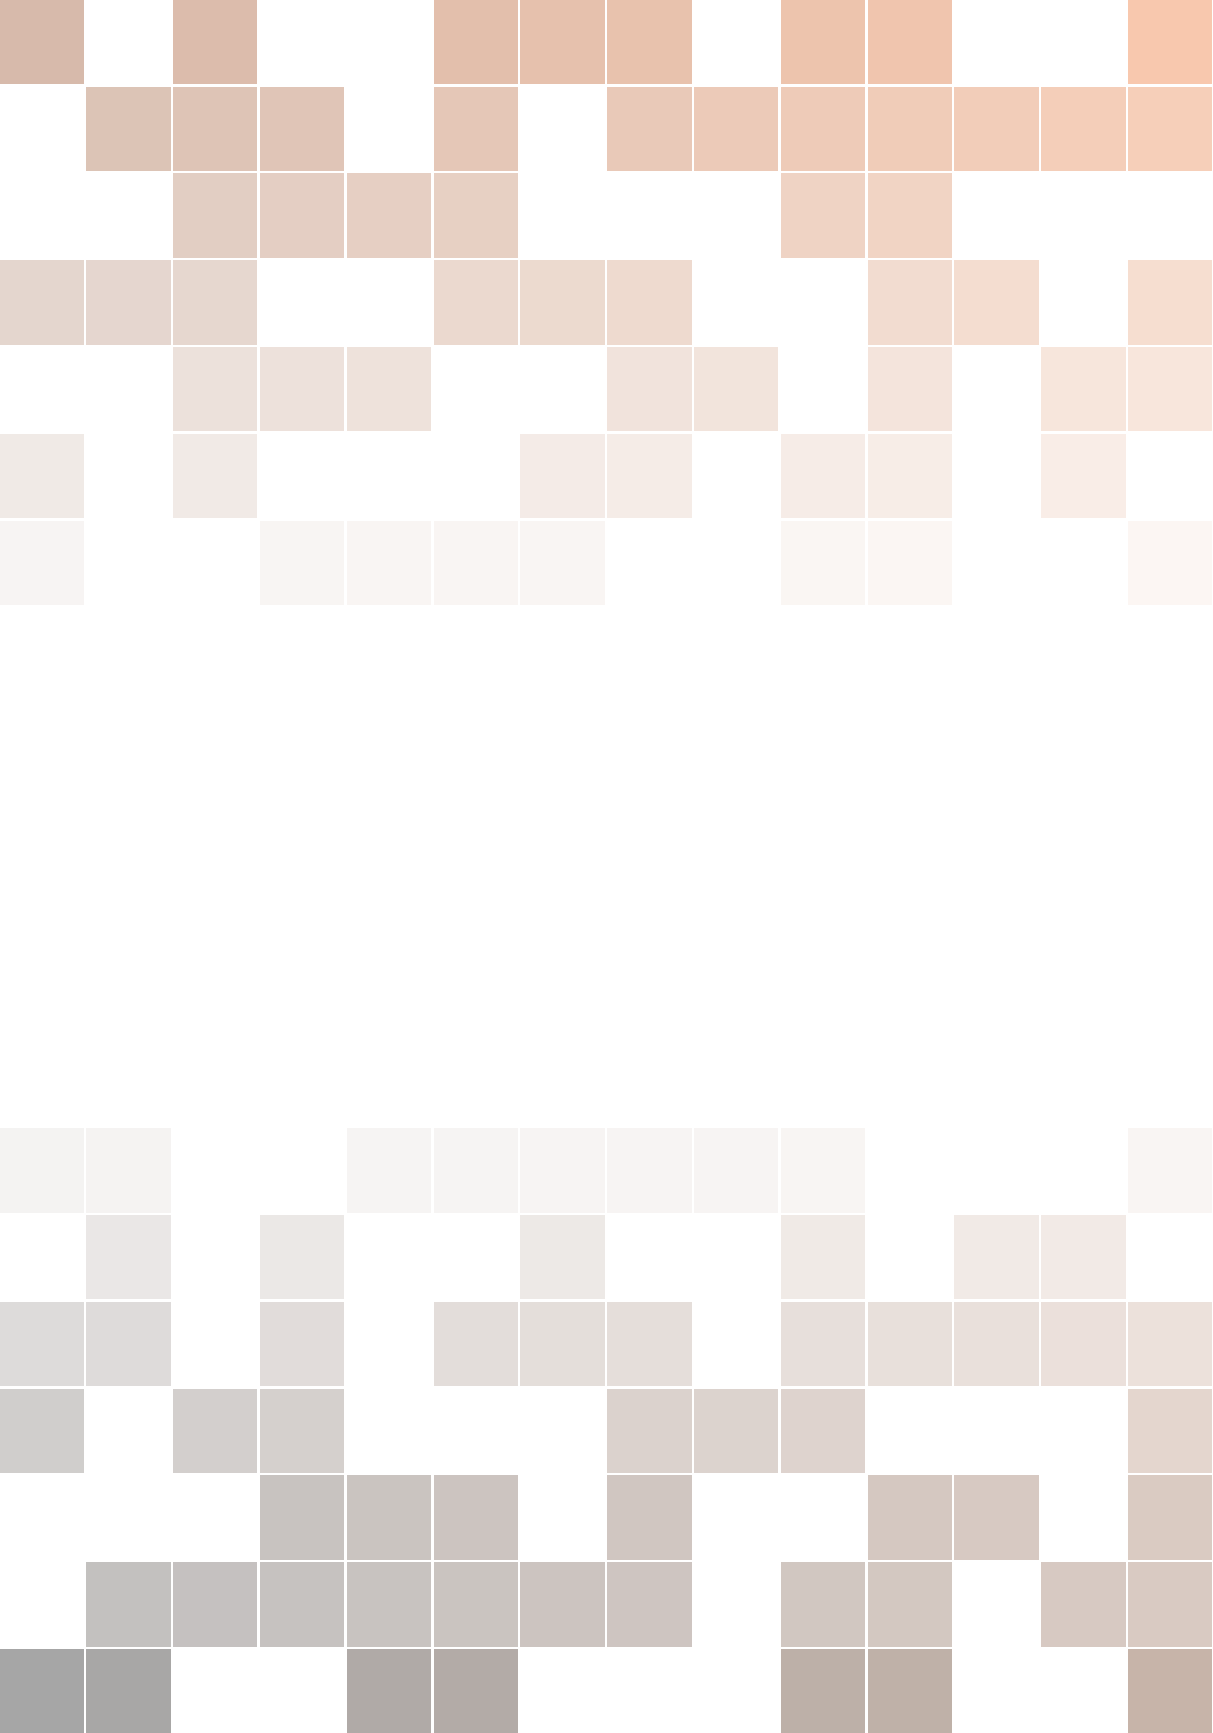
\includegraphics[width=\paperwidth]{background}};
\draw (current page.center) node [fill=ocre!30!white,fill opacity=0.6,text opacity=1,inner sep=1cm]{\Huge\centering\bfseries\sffamily\parbox[c][][t]{\paperwidth}{\centering Álgebra 1\\[15pt] % Book title
{\Large Notas de Aula \semestre/\ano}\\[20pt] % Subtitle
{\huge Jos\'e Ant\^onio O. Freitas}\\
{\large \today}}}; % Author name

\end{tikzpicture}
\vfill
\endgroup

%----------------------------------------------------------------------------------------
%	COPYRIGHT PAGE
%----------------------------------------------------------------------------------------

\newpage
~\vfill
\thispagestyle{empty}

\noindent \ccbyncsa\ Este texto est\'a licenciado sob uma \textbf{Licen\c{c}a Creative Commons Atribui\c{c}\~ao-N\~aoComercial-CompartilhaIgual 3.0 Brasil} \href{http://creativecommons.org/licenses/by-nc-sa/3.0/br/deed.pt\_BR}{\textit{http://creativecommons.org/licenses/by-nc-sa/3.0/br/deed.pt\_BR}}\\ % Copyright notice

%----------------------------------------------------------------------------------------
%	TABLE OF CONTENTS
%----------------------------------------------------------------------------------------

\usechapterimagefalse % If you don't want to include a chapter image, use this to toggle images off - it can be enabled later with \usechapterimagetrue

\chapterimage{chapter_head_1.pdf} % Table of contents heading image

\pagestyle{empty} % No headers

\tableofcontents % Print the table of contents itself

\cleardoublepage % Forces the first chapter to start on an odd page so it's on the right

\pagestyle{fancy} % Print headers again

%!TEX program = xelatex
%!TEX root = Algebra1.tex
%%Usar makeindex -s indexstyle.ist arquivo.idx no terminal para gerar o {\'\i}ndice remissivo agrupado por inicial
%%Ap\'os executar pdflatex arquivo
\begin{center}
\Huge \textbf{Pref{\'a}cio}
\end{center}
\hspace{0,5cm}Essas notas de Aula s{\~a}o referentes {\`a} mat{\'e}ria {\'A}lgebra 1,
ministrada na UnB - Universidade de Bras{\'\i}lia - durante o 2º Semestre de 2010
pelo professor Jos{\'e} Ant{\^o}nio de O. Freitas, Departamento de Matem{\'a}tica. Tais
notas foram transcritas e editadas pelo graduando em Ci{\^e}ncias Econ{\^o}micas
Luiz Eduardo Sol R. da Silva\footnote{luizeduardosol@hotmail.com}.

{\'E} livre a reprodu{\c c}{\~a}o, distribui{\c c}{\~a}o e edi{\c c}{\~a}o deste material, desde que citadas as suas fontes e autores. Cr{\'\i}ticas e sugest{\~o}es s{\~a}o bem vindas.
\vspace{20cm}




\begin{center} \textbf{\Large Nota{\c c}{\~o}es e express{\~o}es}
\end{center}
\begin{minipage}[l]{0,5\textwidth}
\begin{itemize}
\item $\neg$ N{\~a}o
\item $\forall$ Para todo
\item $/$ Tal que
\item $|$ Divide
\item $\Rightarrow$ Implica
\item $\in$ Pertence
\item $\emptyset$ Vazio
\item $\subseteq$ Contido ou igual a
\item $\supseteq$ Cont{\'e}m ou igual a
\item $\wedge$ E
\item $\vee$ Ou
\item $=$ Igual
\item $\neq$ Diferente
\item $\mathbb{Z}$ N{\'u}meros Inteiros
\item $\mathbb{R}$ N{\'u}meros Reais
\item $\cap$ Intersec{\c c}{\~a}o
\item $>$ Maior que
\item $\geq$ Maior ou igual a
\item $\displaystyle\bigcup_{i=1}^{n}$ Uni{\~a}o de $n$ conjuntos
\item $\displaystyle\bigsqcup_{i=1}^{n}$ Uni{\~a}o disjunta de $n$ conjuntos


\end{itemize}
\end{minipage}
\begin{minipage}[r]{0,5\textwidth}
\begin{itemize}

\item $\leftrightarrow$ Se, e somente se
\item $\veebar$ Ou...,ou..., mas nunca ambos
\item $\rightarrow$ Se,... ent{\~a}o...
\item $\exists$ Existe
\item $\Leftrightarrow$ Equivalente a
\item $\notin$ N{\~a}o pertence
\item \# Fim da demonstra{\c c}{\~a}o
\item $\mathbb{N}$ N{\'u}meros Naturais
\item $\mathbb{Q}$ N{\'u}meros Racionais
\item $\nsubseteq$ N{\~a}o cont{\'e}m ou {\'e} igual a
\item $\cup$ Uni{\~a}o
\item $\sqcup$ Uni{\~a}o Disjunta
\item $<$ Menor que
\item $\leq$ Menor ou igual a
\item $\displaystyle\bigcap_{i=1}^{n}$ Intersec{\c c}{\~a}o de $n$ conjuntos
\item Q.E.D. (\textit{Quod Erat Demonstrandum}): Como se queria demonstrar
\item P.B.O.: Princ{\'\i}pio da boa ordena{\c c}{\~a}o
\item H.I.: Hip{\'o}tese de Indu{\c c}{\~a}o
\item \textit{Mutatis Mutandis}:  Mudando o que tem que ser mudado

\end{itemize}
\end{minipage}
%!TEX program = xelatex
%!TEX root = Algebra_1.tex
%%Usar makeindex -s indexstyle.ist arquivo.idx no terminal para gerar o {\'\i}ndice remissivo agrupado por inicial
%%Ap\'os executar pdflatex arquivo
\chapter{Conceitos B\'asicos} % (fold)
\label{cha:conceitos_basicos}

\begin{definicao}
	Uma \textbf{proposi\c{c}\~ao} \'e todo conjunto de palavras ou s{\'\i}mbolos ao qual podemos atribuir um \textbf{valor l\'ogico}.
\end{definicao}

\begin{definicao}
	Diz-se que o \textbf{valor l\'ogico} de uma proposi\c{c}\~ao \'e ``verdade'' (V) se a proposi\c{c}\~ao \'e verdadeira ou ``falsidade'' (F) se a proposi\c{c}\~ao \'e falsa.
\end{definicao}

\begin{exemplos}
	Julgue se as seguintes sentenças são ou não proposições:
	\begin{enumerate}[label={\arabic*})]
		\item Todo número primo é ímpar.
		Essa setença é uma proposição de valor lógico "Falsidade."
		\item $x^2 + y^2 \ge 0$ para todos $x$, $y \in \real$.
		Esse setença é uma proposição de valor lógico "Verdade".
		\item Amanhã irá chover.
		Essa sentença não é uma proposição. Não é possível atribuir um valor lógico a ela.
	\end{enumerate}

\end{exemplos}

\section{Princ{\'\i}pio da n\~ao contradi\c{c}\~ao e do terceiro exclu{\'\i}do} % (fold)
\label{sec:principio_da_nao_contradicao_e_do_3}
\begin{enumerate}[label={\roman*})]
	\item Uma proposi\c{c}\~ao n\~ao pode ser verdadeira e falsa ao mesmo tempo.
	\item Toda proposi\c{c}\~ao ou \'e verdadeira ou \'e falsa, isto \'e, verifica-se sempre um destes casos e nunca um terceiro.
\end{enumerate}

Assim esses princ{\'\i}pios afirmam que:
\begin{center}
	``Toda proposi\c{c}\~ao tem um, e um s\'o, dos valores l\'ogicos \textbf{verdade} ou \textbf{falsidade}.''
\end{center}

De modo geral vamos trabalhar com proposi\c{c}\~oes da forma:
\begin{enumerate}[label={\roman*})]
	\item Se $\mathcal{H}$, ent\~ao $\mathcal{T}$.

	Aqui $\mathcal{H}$ \'e chamado de hip\'otese e $\mathcal{T}$ de tese. Neste tipo de proposi\c{c}\~ao iremos admitir que $\mathcal{H}$ \'e uma verdade e precisaremos provar que $\mathcal{T}$ \'e verdade. Ou seja precisamos construir um argumento que justifique $\mathcal{T}$ ser verdadeira \`a partir do fato de $\mathcal{H}$ ser verdadeira.

	\item $\mathcal{H}$ se, e somente se, $\mathcal{T}$ ou $\mathcal{H}$ se, e s\'o se, $\mathcal{T}$.

	Esse tipo de proposi\c{c}\~ao ser\'a decomposta em duas proposi\c{c}\~oes no formato anterior. Isto \'e:
	\begin{enumerate}[label={\alph*})]
		\item Se $\mathcal{H}$, ent\~ao $\mathcal{T}$.
		\item Se $\mathcal{T}$, ent\~ao $\mathcal{H}$.
	\end{enumerate}

	No primeiro caso admitimos $\mathcal{H}$ verdadeira e provamos que $\mathcal{T}$ tamb\'em \'e verdadeira e no segundo caso admitimos que $\mathcal{T}$ \'e verdadeira e provamos que $\mathcal{H}$ \'e verdadeira.
\end{enumerate}
% section pr{\'\i}ncipio_da_n\~ao_contradi\c{c}\~ao_e_do_3 (end)

% chapter conceitos_b\'asicos (end)

\chapter{No{\c c}{\~o}es de Teoria de Conjuntos}
\section{Conceitos b{\'a}sicos}

Um conjunto {\'e} uma ``cole{\c c}{\~a} o'' ou ``fam{\'\i}lia'' de elementos.

Usaremos letras mai{\'u}sculas do alfabeto para denotar os conjuntos e denotaremos elementos de um dado conjunto por letras min{\'u}sculas do alfabeto.

Dado um conjunto $A$, para indicar o fato de que $x$ {\'e} um elemento de $A$, escrevemos:
\[
x \in A.
\]

Para dizer que um elemento $x$ n{\~a}o pertence ao conjunto $A$, escrevemos:
\[
x \notin A.
\]

Um conjunto sem elementos {\'e} chamado de \textbf{conjunto vazio}. Tal conjunto {\'e} denotado por $\emptyset$.

Dado um conjunto $A$ e $x$ um elemento, ocorre sempre o uma das seguintes situa\c{c}\~oes:
\[
x \in A \mbox{ ou } x \notin A.
\]

Al{\'e}m disso, para dois elementos $x$, $y \in A$, ocorre exatamente uma das seguinte situa\c{c}\~oes:
\[
x = y \mbox{ ou } x \neq y.
\]

\section{Descri{\c c}{\~a}o de um conjunto}

Um conjunto $A$ pode ser dado pela simples listagem dos seus elementos, como por exemplo:
\begin{align*}
	A= \{1,2,3,4,5\}\\
	B = \{verdade, falso\}.
\end{align*}

Um conjunto tamb{\'e}m pode ser dado pela descri{\c c}{\~a}o das propriedades dos seus elementos, como por exemplo:
\[
A = \{n \mid n \mbox{ \'e m{\'u}ltiplo de } 2\} = \{2,4,6,...\}.
\]

\section{Alguns conjuntos importantes}
\begin{enumerate}[label={\arabic*})]
	\item $\n = \{0,1,2,3,...\}$ o conjunto do n{\'u}meros naturais.
	\item $\z = \{...,-2,-1,0,1,2,...\}$ o conjunto dos n{\'u}meros inteiros.
	\item $\n_0 = \{0,1,2,3,...\}$ o conjunto dos n{\'u}meros inteiros n{\~a}o negativos.
	\item $\real $ o conjunto dos n{\'u}meros reais.
	\item $\real^*$ o conjunto dos n{\'u}meros reais n{\~a}o nulos.
	\item $\rac = \left\{\dfrac{p}{q} \mid p,q \in \z, q \neq 0 \right\}$ o conjunto dos n{\'u}meros racionais.
\end{enumerate}

\section{Propriedades dos conjuntos}

\begin{definicao}
	Dados dois conjuntos $A$ e $B$, dizemos que $A$ e $B$ s{\~a}o \textbf{iguais} se, e somente se, eles t{\^e}m os mesmos elementos. Ou seja, para todo $x \in A$ temos que $x \in B$ e para todo $y \in B$ temos $y \in A$.
\end{definicao}

Se $A$ e $B$ s{\~a}o iguais, escrevemos $A = B$
\begin{align*}
	\{1,2,3,4\} &= \{3,2,1,4\}\\
	\{1,2,3\} &\ne \{2,3\} 
\end{align*}
	
\begin{definicao}
	Se $A$ e $B$ s{\~a}o dois conjuntos, dizemos que $A$ {\'e} um \textbf{subconjunto} de $B$ ou que $A$ \textbf{est\'a contido} em $B$ ou que $B$ \textbf{cont\'em} $A$ se todo elemento de $A$ for elemento de $B$. Ou seja, se para todo elemento $x \in A$, temos $x \in B$. Nesse caso, escrevemos $A \subseteq B$ ou $B \supseteq A$.
\end{definicao}


Caso $A$ seja um subconjunto de $B$ mas n{\~a}o {\'e} igual a $B$, escrevemos:
\[
A \subsetneq B.
\]

Nesse caso, dizemos que $A$ {\'e} um \textbf{subconjunto pr{\'o}prio} de $B$.

Para dizer que $A$ n{\~a}o est{\'a} contido em $B$, escrevemos $A \nsubseteq B$

Usando a defini\c{c}\~ao de contin\^encia de conjuntos podemos definir igualdade de conjuntos da seguinte forma:
\begin{center}
	\textbf{dois conjuntos $A$ e $B$ s\~ao iguais se, e somente se, $A \subseteq B$ e $B \subseteq A$}.
\end{center}

Ou seja,
\begin{center}
	\textbf{se $A = B$ ent{\~a}o $A \subseteq B$ e $B \subseteq A$}.
\end{center}

Além disso,
\begin{center}
	\textbf{se $A \subseteq B$ e $B \subseteq A$, ent{\~a}o $A = B$}.
\end{center}

Quando $A$ e $B$ n{\~a}o s{\~a}o iguais, escrevemos $A \neq B$. Para que $A \neq B$ devemos ter $A \nsubseteq B$ ou $B \nsubseteq A$. Isto é, precisamos encontrar algum elemento $x \in A$ tal que $x \notin B$ ou então encontrar $y \in B$ tal que $y \notin A$.

\begin{proposicao}
	Dados três conjuntos $A$, $B$ e $C$ temos:
	\begin{enumerate}[label={\roman*})]
		\item $A\subseteq A$ (Reflexividade)
		\item Se $A\subseteq B \mbox{ e } B\subseteq A$, ent{\~a}o $A=B$. (Antissimetria)
		\item Se $A\subseteq B$ e $B\subseteq C$, ent{\~a}o $A\subseteq C$. (Transitividade)
	\end{enumerate}
\end{proposicao}


Considere os seguintes conjuntos:
\begin{align*}
	A &= \{ n \in \n \mid n \mbox{ {\'e} m{\'u}ltiplo de } 2\} = \{2,4,6,...\}\\
	B &= \{n \in \n \mid n \mbox{ {\'e} m{\'u}ltiplo de } 3\} = \{3,6,9,...\}.
\end{align*}


Neste caso, $2 \in A$ e $2 \notin B$, logo $A \nsubseteq B$. Por outro lado, $3 \in B$ e $3 \notin A$ e com isso $B \nsubseteq A$. Portanto, dados dois conjuntos $A$ e $B$, nem sempre temos $A \subseteq B$ ou $B \subseteq A$.

\begin{proposicao} 
	Seja $A$ um conjunto. Ent{\~a}o $ \emptyset \subseteq A$.
\end{proposicao}
\begin{prova}
	Suponha que $\emptyset \nsubseteq A$. Logo existe $x \in \emptyset$ tal que $x \notin A$. Mas por defini{\c c}{\~a}o, o conjunto vazio n{\~a}o cont{\'e}m elementos. Logo a exist\^encia de $x \in \emptyset$ {\'e} uma contradi{\c c}{\~a}o. Tal contradi\c{c}\~ao surgiu por termos suposto que $\emptyset \nsubseteq A$. Portanto, $\emptyset \subseteq A$, como quer{\'\i}amos demonstrar.
\end{prova}

\section{Rela{\c c}{\~o}es entre conjuntos}

\begin{definicao}\label{intersecao_conjunto}
Sejam $A$ e $B$ dois conjuntos. Definimos a \textbf{intersec{\c c}{\~a}o} de $A$ e $B$ como sendo o conjunto $A \cap B$ cujos elementos pertencem ao conjunto $A$ e $B$ simultaneamente. Assim,
\[
A \cap B = \{x \mid x \in A\mbox{ e }  x \in B\}.
\]
\end{definicao}

\begin{exemplo}
	Sejam $A = \{1, 2, 3\}$, $B = \{2, 3, 4\}$ e $C = \{r, s, t\}$. Então
	\begin{align*}
		A \cap B &= \{2, 3\}\\
		A \cap C &= \emptyset.
	\end{align*}
\end{exemplo}

\begin{definicao}\label{unicao_conjuntos}
Sejam $A$ e $B$ dois conjuntos. Definimos a \textbf{uni{\~a}o} de $A$ com $B$ como sendo o conjunto $A \cup B$, cujos elementos pertencem ao conjunto $A$ ou ao conjunto $B$. Assim,
\[
A \cup B = \{x \mid x \in A \mbox{ ou } x \in B\}.
\]
\end{definicao}

\begin{exemplo}
	Sejam $A = \{1, 2, 3\}$, $B = \{2, 3, 4\}$ e $C = \{r, s, t\}$. Então
	\begin{align*}
		A \cup B &= \{1,2,3,4\}\\
		A \cup C &= \{1,2,3,r,s,t\}.
	\end{align*}
\end{exemplo}

\begin{proposicao} Sejam $A$ e $B$ dois conjuntos. Ent{\~a}o:
	\begin{enumerate}[label={\roman*})]
		\item $(A \cap B) \subseteq A$;
		\item $(A \cap B) \subseteq B$;
		\item $A \subseteq A \cup B$;
		\item $B \subseteq A \cup B$.
	\end{enumerate}
\end{proposicao}
\begin{prova}
	Para provar a primeira afirmação seja $x \in A \cap B$ um elemento qualquer. Da defini\c{c}\~ao de interse\c{c}\~ao de conjuntos, Definição \ref{intersecao_conjunto}, temos $x \in A$ e $x \in B$. Assim podemos afirmar com certeza que $x \in A$. Logo todo elemente de $A \cap B$ também está em $A$, ou seja, $A \cap B \subseteq A$. De modo análogo prova-se a segunda afirmação sobre interseção.

	Para a terceira afirmação, seja $x \in A$. Da definição de união de conjuntos, Definição \ref{unicao_conjuntos}, segue que $x \in A \cup B$. Logo todo elemento de $A$ também está em $A \cup B$, ou seja, $A \subseteq (A \cup B)$. De modo análogo prova-se a quarta afirmação.
\end{prova}

O conceito de uni{\~a}o ($ \cup $) e intersec{\c c}{\~a}o ($ \cap $) pode ser estendido para mais de dois conjuntos.

\begin{definicao}
Sejam $A_{1}$, \dots, $A_{n}$ conjuntos. Ent{\~a}o
\[
A_{1} \cup A_{2} \cup \cdots \cup A_{n}= \displaystyle\bigcup_{k=1}^n A_{k}
\]
{\'e} o conjunto dos elementos $x$ tais que $x$ pertence a pelo menos um dos conjuntos $A_{1}$, \dots, $A_{n}$. Agora,
\[
A_{1} \cap \cdots \cap A_{n} = \displaystyle\bigcap_{k=1}^{n}A_{k}
\]
{\'e} o conjunto dos elementos $x$ que pertencem a todos os conjuntos $A_{1}$, \dots, $A_{n}$ simultaneamente.
\end{definicao}

\begin{definicao}
	Sejam $A$ e $B$ conjuntos. Se $A \cap B = \emptyset$, dizemos que $A$ e $B$ s{\~a}o \textbf{conjuntos disjuntos}.	
\end{definicao}


Sejam $A$ e $B$ conjuntos tais que $C = A \cup B$ e $A \cap B = \emptyset$. Neste caso dizemos que $C$ {\'e} uma \textbf{uni{\~a}o disjunta} de $A$ e $B$. Denotamos tal fato por
\[
C = A \sqcup B.
\]

\begin{proposicao} Sejam $A,\ B$ e $C$ tr{\^e}s conjuntos, ent{\~a}o:
	\begin{enumerate}[label={\roman*})]
		\item $A\cap(B\cup C)=(A\cap B)\cup(A\cap C)$
		\item $A\cup(B\cap C)=(A\cup B)\cap(A\cup C)$
	\end{enumerate}
\end{proposicao}
\begin{prova}
	\begin{enumerate}[label={\roman*})]
		\item Precisamos mostrar que
		\begin{enumerate}[label={\roman*})]
			\item $A\cap(B\cup C)\subseteq(A\cap B)\cup(A\cap C)$;\label{intersecao_unicao_1}
			\item $(A\cap B)\cup(A\cap C)\subseteq A\cap(B\cup C).$\label{intersecao_unicao_2}
		\end{enumerate}

		Para provar \ref{intersecao_unicao_1} seja $x\in A \cap (B \cup C)$. Logo $x\in A$ e $x\in B\cup C$. Agora, de $x\in B\cup C$, segue que $x\in B$ ou $x\in C$. Suponha que $x\in B$. Como $x\in A$ e $x \in B$, ent\~ao $x\in A\cap B$. Assim, $x\in(A\cap B)\cup(A\cap C)$, ou seja, $A\cap(B\cup C)\subseteq(A\cap B)\cup(A\cap C)$. Por outro lado, se $x\in C$, como $x\in A$, ent{\~a}o $x\in A\cap C$ e da{\'\i} $x\in(A\cap B)\cup(A\cap C)$, logo $A\cap(B\cup C)\subseteq(A\cap B)\cup(A\cap C)$.

		Portanto,
		\[
			A\cap(B\cup C)\subseteq(A\cap B)\cup(A\cap C).
		\]

		Agora para provar \ref{intersecao_unicao_2}, seja $x\in(A\cap B)\cup(A\cap C)$. Da{\'\i}, $x\in A\cap B$ ou $x\in A\cap C$. Suponha que $x\in A\cap B$. Assim, $x\in A$ e $x\in B$. Como $x\in B$, segue que $x\in B\cup C$ e ent{\~a}o $x\in A\cap(B\cup C)$, ou seja, $(A\cap B)\cup(A\cap C)\subseteq A\cap(B\cup C)$. Agora, suponha que $x\in A\cap C$. Com isso $x\in A$ e $x\in C$. Desse modo, $x\in B\cup C$ e ent{\~a}o $x\in A\cap(B\cup C)$ e da{\'\i}
		\[
			(A\cap B)\cup(A\cap C)\subseteq A\cap(B\cup C).
		\]

		Portanto
		\[
			A\cap(B\cup C)=(A\cap B)\cup(A\cap C),
		\]
		como quer{\'\i}amos.
		\item An\'aloga ao caso anterior.
	\end{enumerate}
\end{prova}

\begin{definicao}
	Dados dois conjuntos $A$ e $B$, definimos a \textbf{diferen{\c c}a} dos conjuntos $A$ e $B$, denotada por $A-B$ ou $A\backslash B$ como sendo o conjunto
	\[
		A - B = \{x \mid x \in A \mbox{ e } x \notin B\}.
	\]
\end{definicao}

\begin{exemplos}
	\begin{enumerate}[label={\arabic*})]
		\item Se $A=\{1,2,3,5,4\}$, $B=\{2,3,6,8\}$, então
		\begin{align*}
			A - B &= \{1,4,5\}\\
			B - A &=\{6,8\}.
		\end{align*}
		\item Se $A=\{2,4,6,8,10,...\}$, $B=\{3,6,9,12,15,...\}$, então
		\begin{align*}
		 	A - B &= \{2,4,8,10,14,16,...\}\\
		 	B - A &= \{3,9,15,21,...\}
		 \end{align*}
	\end{enumerate}
	
\end{exemplos}

\begin{proposicao}
	Sejam $A$, $B$ e $C$ conjuntos n\~ao vazios. Ent\~ao
	\[(A \cup B) - C = (A - C) \cup (B - C).\]
\end{proposicao}
\begin{prova}
	Segue da defini\c{c}\~ao de diferen\c{c}a de conjuntos.
\end{prova}

\begin{definicao}
Dados dois conjuntos $A$ e $E$ tais que $A\subseteq E$, definimos o \textbf{complementar} de $A$ em $E$, denotado $A^C$ ou $C_E(A)$, como
\[
	C_E(A) = \{ x \in E \mid x \notin A \}.
\]
\end{definicao}

\begin{observacoes}
	\begin{enumerate}[label={\arabic*})]
		\item Se $A = E$, ent{\~a}o $C_A(A) = \{ x \in A \mid x \notin A \} = \emptyset$.
		\item $(A^C)^C = \{x \in E \mid x \notin A^C\} = \{ x \in E \mid x \in A \} = A$
	\end{enumerate}
	
\end{observacoes}

\begin{exemplo}
	Sejam $A = \{1,2,3,4\}$ e $E = \{1,2,3,5,4,0,8,9\}$. Primeiro note que $A \subseteq E$, daí
	\[
			A^C = C_E(A) = \{0,5,8,9\}.
	\]
\end{exemplo}

\begin{proposicao}
	Sejam $A$, $B$ e $E$ conjuntos. Se $A\subseteq B\subseteq E$, ent{\~a}o $C_E(B)\subseteq C_E(A)$.
\end{proposicao}
\begin{prova}
	Seja $x \in C_E(B)$. Assim $x\notin B$ e como $A \subseteq B$, ent\~ao $x \notin A$. Da{\'\i} por defini\c{c}\~ao $x\in C_E(A)$, ou seja, $C_E(B) \subseteq C_E(A)$.
\end{prova}

\begin{proposicao} Sejam $A$, $B$ e $E$ tr{\^e}s conjunto tais que $A\subseteq E$ e $B\subseteq E$. Ent{\~a}o:
\begin{enumerate}[label={\roman*})]
	\item $(A\cup B)^C = A^C\cap B^C$
	\item $(A\cap B)^C = A^C\cup B^C$
\end{enumerate}
\end{proposicao}
\begin{prova}
	\begin{enumerate}[label={\roman*})]
		\item Seja $x \in (A\cup B)^C$. Logo $x\notin A\cup B$, assim $x\notin A$ e $x\notin B$. Da{\'\i}, $x\in A^C$ e $x\in B^C$, isto {\'e}, $x\in A^C\cap B^C$. Desse modo,
		\begin{equation}\label{complementar_uniao-1}
			(A\cup B)^C \subseteq A^C\cap B^C.
		\end{equation}

		Por outro lado, se $x\in A^C\cap B^C$, ent{\~a}o $x\in A^C$ e $x\in B^C$. Com isso, $x\notin A$ e $x\notin B$, ou seja, $x\notin A\cup B$, logo $x\in (A\cup B)^C$. Desse modo
		\begin{equation}\label{complementar_uniao-2}
			A^C\cap B^C\subseteq(A\cup B)^C.
		\end{equation}

		Portanto, de \eqref{complementar_uniao-1} e \eqref{complementar_uniao-2} temos
		\[
			(A\cup B)^C = A^C\cap B^C.
		\]

		\item Seja $x \in (A\cap B)^C$. Logo $x\notin A\cap B$, assim $x\notin A$ ou $x\notin B$. Ent\~ao $x\in A^C$ ou $x\in B^C$, isto {\'e}, $x\in A^C\cup B^C$. Desse modo,
		\begin{equation}\label{complementar_intersecao-1}
			(A\cap B)^C \subseteq A^C\cup B^C.
		\end{equation}

		Por outro lado, se $x\in A^C\cup B^C$, ent{\~a}o $x\in A^C$ ou $x\in B^C$. Da{\'\i}, $x\notin A$ ou $x\notin B$, ou seja, $x\notin A\cap B$, logo $x\in (A\cap B)^C$. Desse modo
		\begin{equation}\label{complementar_intersecao-2}
			A^C\cup B^C\subseteq(A\cap B)^C.
		\end{equation}

		Portanto, de \eqref{complementar_intersecao-1} e \eqref{complementar_intersecao-2} temos
		\[
			(A\cap B)^C = A^C\cup B^C.
		\]
	\end{enumerate}
\end{prova}

\begin{definicao}
	Dados dois conjuntos $A$ e $B$, definimos o \textbf{produto cartesiano} de $A$ por $B$ como sendo o conjunto
	\[
		A \times B = \{(x,y) \mid x\in A, y\in B\}.
	\]
\end{definicao}

Dados $(x,y)$, $(z,t) \in A\times B$, temos
\begin{center}
	\textbf{$(x,y) = (z,t)$ se, e somente se, $x = z$ e $y = t$}.
\end{center}

\begin{exemplo}\label{exemplo_produto_cartesiano}
	Sejam $A = \{1,2\}$ e $B = \{3,4\}$. Então
	\begin{align*}
		A \times B &= \{(1,3), (1,4), (2,3), (2,4)\}\\
		B \times A &= \{(3,1), (3,2), (4,1), (4,2)\}
\end{align*}
\end{exemplo}

\begin{observacao}
	Do Exemplo \eqref{exemplo_produto_cartesiano} vemos que em geral $A \times B \neq B\times A$.
\end{observacao}

\begin{definicao}
	Para qualquer conjunto $A$, indicamos por $\mathcal{P}(A)$ o conjunto
	\[
		\mathcal{P}(A) = \{ X \mid X\subseteq A\}
	\]
	que \'e chamado de \textbf{conjunto das partes} de $A$.
\end{definicao}

Os elementos desse conjunto s{\~a}o todos os subconjuntos de $A$. Dizer que $Y\in \mathcal{P}(A)$ significa que $Y \subseteq A$. Particularmente, temos $\emptyset\in \mathcal{P}(A)$ e $A\in \mathcal{P}(A)$.

\begin{exemplos}
	\begin{enumerate}[label={\arabic*})]
		\item $A = \emptyset$, $\mathcal{P}(A) = \{\emptyset\}$;
		\item $B = \{x\}$, $\mathcal{P}(B) = \{\emptyset, \{x\}\}$;
		\item $C = \{a,b,c\}$, $\mathcal{P}(C)=\{\emptyset, \{a\}, \{b\},\{c\},\{a,b\},\{a,c\},\{b,c\},C\}$;
		\item $D=\real$, $\mathcal{P}(D)=\{X\mid X \subseteq \real\}$, por exemplo $\rac\in \mathcal{P}(D)$.
	\end{enumerate}	
\end{exemplos}
%!TEX program = xelatex
%!TEX root = Algebra_1.tex
%%Usar makeindex -s indexstyle.ist arquivo.idx no terminal para gerar o índice remissivo agrupado por inicial
%%Após executar pdflatex arquivo
% \chapter{Relações e Funções}
\chapter{Relações}
% \section{Relações}
% \subsubsection{Definição}
% Sejam A e B dois conjuntos não vazios. Os subconjuntos de AxB são chamados relações, ou seja, uma relação em AxB é um subconjunto desse produto cartesiano.

% Quando $R$ é uma relação em $A \times B$, também dizemos que $R$ é uma relação de A em B.

% Exemplos:
% \begin{enumerate}[label={\arabic*})]
% \item Se A=\{0,1\} e B=\{-1,0,1\}, então AxB=\{(0,-1),(0,0),(0,1),(1,-1),(1,0),(1,1,)\}\\
% São exemplos de relações:\\
% $R_{1}=\{(0,1)\}$\\
% $R_{2}=\emptyset$\\
% $R_{3}=\{(1,-1),(1,1)\}$\\
% $R_{4}=A$x$B$
% \item Se $A=B=\mathbb{R}$, então AxB é o conjunto formado por todos pares ordenados de números reais. Um exemplo de relação em $\mathbb{R}$x$\mathbb{R}$ é o conjunto:\\
% $R=\{(x,y)\in \mathbb{R}$x$\mathbb{R}/ y\geq 0\}$
% \end{enumerate}

\section{Relações de equivalência}

\begin{definicao}\label{definicao_relacao_equivalencia}
    Seja $A$ um conjunto não vazio e $R\subseteq A \times A$. Dizemos que $R$ é uma \textbf{relação de equivalência} se:
    \begin{enumerate}[label={\roman*})]
        \item Para todo $x \in A$, $(x,x) \in R$. \textit{(Propriedade Reflexiva)}
        \item Se $(x, y) \in R$, então $(y, x) \in R$. \textit{(Propriedade Simétrica)}
        \item Se $(x, y) \in R$ e $(y, z) \in R$, então $(x, z)\in R$. \textit{(Propriedade Transitiva)}
    \end{enumerate}
\end{definicao}

Quando $R\subseteq A \times A$ é uma relação de equivalência, dizemos que $R$ é uma relação de equivalência em $A$. Quando dois elementos $x$, $y \in A$ são tais que $(x,y) \in R$, dizemos que $x$ e $y$ \textbf{são relacionados} ou que $x$ e $y$ \textbf{estão relacionados}.

\begin{exemplos}\label{exemplos_relacoes_equivalencia}
    \begin{enumerate}[label={\arabic*})]
        \item Seja A=\{1,2,3,4\}. Temos
        \begin{align*}
            A\times A = &\{(1,1);(1,2);(1,3);(1,4);(2,1);(2,2);(2,3);(2,4);\\ &(3,1);(3,2);(3,3);(3,4);(4,1);(4,2);(4,3);(4,4)\}.
        \end{align*}
        Quais dos seguintes conjuntos são exemplos de relações de equivalência?
        \begin{itemize}
            \item $R_{1}= A\times A$
            \item $R_{2}=\{(1,1);(2,2);(3,3)\}$
            \item $R_{3}=\{(1,1);(2,2);(3,3);(4,4);(1,2);(2,1)\}$
            \item $R_{4}=\{(1,1);(2,2);(3,3);(4,4)\}$
            \item $R_{5}=\{(1,1);(2,2);(3,3);(4,4);(1,2);(2,1);(2,4);(4;2)\}$
        \end{itemize}
        \begin{solucao}
            $R_2$ não é relação de equivalência pois $(4,4) \notin R_2$.

            $R_5$ não é relação de equivalência pois, por exemplo, $(1,4) \notin R_5$.

            Os demais são exemplos de relações de equivalência.
        \end{solucao}

        \item Seja $A = \z$ e $R\subseteq \z\times \z$ definida por $R = \{(x,y)\in \z \times \z \mid x = y\}$.
        Então $R$ é uma relação de equivalência.
        \begin{solucao}
            De fato,
            \begin{itemize}
                \item Para todo $x \in \z$ temos $x = x$ daí $(x,x) \in R$.
                \item Se $(x,y)\in R$, então pela definição de $R$ temos $x = y$. Logo $y = x$ e então $(y,x)\in R$.
                \item Se $(x,y) \in R$ e $(y,z) \in R$, então  $x = y$ e $y = z$. Logo $x = z$ e assim $(x,z)\in R$ como queríamos.
            \end{itemize}
            Portanto $R$ é uma relação de equivalência sobre $\z$.
        \end{solucao}

        \item Seja $A = \z$ e tome $R = \{(x,y)\in \z \times \z \mid x - y = 2k, \mbox{ para algum } k \in \z\}$. Mostre que $R$
        é uma relação de equivalência sobre $\z$.
        \begin{solucao}
            De fato,
            \begin{itemize}
                \item Para todo $x\in\z$ temos $x - x = 2\cdot0$ e com isso $(x,x) \in R$.
                \item Se $(x,y) \in R$ então existe $k \in \z$ tal que $x - y = 2k$. Agora $y - x = -(x - y) = -2k = 2 (-k)$
                e como $-k \in \z$ segue que $(y,x) \in R$.
                \item Se $(x,y) \in R$ e $(y,z) \in R$, então existem $k$, $l\in \z$ tais que $x - y = 2k$ e $y - z = 2l$.
                Somando essas duas equações obtemos
                \begin{align*}
                    (x - y) + (y - z) &= 2k + 2l\\
                    x - z &= 2(k + l)
                \end{align*}
                e como $k + l \in \z$ segue que $(x,z) \in \z$.
            \end{itemize}
            Assim $R$ é uma relação de equivalência.
        \end{solucao}
    \end{enumerate}
\end{exemplos}
\begin{observacoes}
    Seja $R$ uma relação de equivalência em $A$, isto é, $R \sub A \times A$.
    \begin{enumerate}[label={\arabic*})]
        \item  Para dizermos que $(x,y) \in R$ usaremos a notação $x\equiv y\ (R)$, que se lê ``$x$ é equivalente a $y$ módulo $R$", ou ainda a notação $xRy$, com o mesmo significado anterior.
        \item Em alguns casos vamos utilizar a notação $\sim$ para representar a relação $R$. Nesse caso, escrevemos $x \sim y$ para dizer que $(x, y) \in R$, ou que, $xRy$.
    \end{enumerate}
\end{observacoes}

Em virtude da observação anterior a definição de relação de equivalência pode ser reescrita como:

\begin{definicao}
    Seja $A$ um conjunto não vazio e $R\subseteq A \times A$. Dizemos que $R$ é uma \textbf{relação de equivalência} se:
    \begin{enumerate}[label={\roman*})]
        \item Para todo $x \in A$, $xRx$. \textit{(Propriedade Reflexiva)}
        \item Se $xRy$, então $yRx$. \textit{(Propriedade Simétrica)}
        \item Se $xRy$ e $yRz$, então $xRz$. \textit{(Propriedade Transitiva)}
    \end{enumerate}
\end{definicao}

\begin{definicao}
    Seja $R$ uma relação de equivalência sobre um conjunto $A$. Dado $b \in A$, chamamos de \textbf{classe de equivalência determinada por $b$ módulo $R$}, denotada por $\overline{b}$ ou $C(b)$, o subconjunto de $A$ dado por
    \[
        \overline{b} = C(b) = \{x \in A \mid (x,b) \in R\} = \{x \in A \mid xRb\}.
    \]
\end{definicao}

\begin{observacao}
    Seja $A \ne \emptyset$ e $R$ uma relação de equivalência sobre $A$. Segue da definição de relação de equivalência que para todo $b \in A$, $\overline{b} \ne \emptyset$ pois $(b,b) \in R$ logo $b \in \overline{b}$.
\end{observacao}

\begin{exemplos}\label{exemplos_classes_equivalencia}
    Do Exemplo \ref{exemplos_relacoes_equivalencia} temos
    \begin{enumerate}[label={\arabic*})]
        \item As classes de equivalência de $R_1$ são:
        \begin{align*}
            \overline{1} &= \{x \in A \mid (x,1) \in R_1\} = \{1,2,3,4\}\\
            \overline{2} &= \{x \in A \mid (x,2) \in R_1\} = \{1,2,3,4\}\\
            \overline{3} &= \{x \in A \mid (x,3) \in R_1\} = \{1,2,3,4\}\\
            \overline{4} &= \{x \in A \mid (x,4) \in R_1\} = \{1,2,3,4\}\\
        \end{align*}
        Nesse caso temos somente uma classe de equivalência.

        \item As classes de equivalência de $R_3$ são:
        \begin{align*}
            \overline{1} &= \{x \in A \mid (x,1) \in R_3\} = \{1,2\}\\
            \overline{2} &= \{x \in A \mid (x,2) \in R_3\} = \{1,2\}\\
            \overline{3} &= \{x \in A \mid (x,3) \in R_3\} = \{3\}\\
            \overline{4} &= \{x \in A \mid (x,4) \in R_3\} = \{4\}\\
        \end{align*}
        Aqui temos três classes de equivalência diferentes.

        \item As classes de equivalência de $R_4$ são:
        \begin{align*}
            \overline{1} &= \{x \in A \mid (x,1) \in R_4\} = \{1\}\\
            \overline{2} &= \{x \in A \mid (x,2) \in R_4\} = \{2\}\\
            \overline{3} &= \{x \in A \mid (x,3) \in R_4\} = \{3\}\\
            \overline{4} &= \{x \in A \mid (x,4) \in R_4\} = \{4\}\\
        \end{align*}
        Aqui temos quatro classes de equivalência diferentes.

        \item Para a relação de equivalência $R = \{(x,y)\in \z \times \z \mid x - y = 2k, \mbox{ para algum } k \in \z\}$ temos:
        \begin{align*}
            \overline{0} &= \{x \in \z \mid xR0 \} = \{x \in \z \mid x - 0 = 2k,\ k \in \z\} \\
            \overline{0} &= \{x \in \z \mid x = 2k,\ k \in \z\} = \{0, \pm 2, \pm 4, \pm 6, \dots\}\\
            \overline{1} &= \{x \in \z \mid xR1 \} = \{x \in \z \mid x - 1 = 2k,\ k \in \z\} \\
            \overline{1} &= \{x \in \z \mid x = 2k + 1,\ k \in \z\} = \{\pm 1, \pm 3, \pm 4, \pm 7, \dots\}\\
        \end{align*}
        Neste caso existem somente duas classes de equivalência. (\textit{Por quê?})
    \end{enumerate}
\end{exemplos}

\begin{proposicao}
    Seja $R$ uma relação de equivalência em um conjunto não vazio $A$. Dados $a$, $b \in A$ temos:
    \begin{enumerate}[label={\roman*})]
        \item se $\overline{a} \cap \overline{b} \ne \emptyset$, então $aRb$.
        \item se  $\overline{a} \cap \overline{b} \neq \emptyset$, então $\overline{a} = \overline{b}$.
    \end{enumerate}
\end{proposicao}
\begin{prova}
    \begin{enumerate}[label={\roman*})]
        \item Como  $\overline{a} \cap \overline{b} \ne \emptyset$, existe um $y \in \overline{a} \cap \overline{b}$, logo $y \in \overline{a}$ e $y \in \overline{b}$. Da definição de classe de equivalência temos $yRa$ e $yRb$. Como $R$ é relação de equivalência temos $aRy$ e $bRy$. Pela propriedade transitiva segue que $aRb$, como queríamos.

        \item Precisamos mostrar que $\overline{a} \sub \overline{b}$ e que $\overline{b} \sub \overline{a}.$ Para a primeira inclusão seja $y \in \overline{a}$. Daí $yRa$. Mas, por hipótese, $\overline{a}\cap\overline{b}\neq\emptyset$, assim pelo item anterior segue que $aRb$. Logo, como $yRa$ e $aRb$, segue que $yRb$, ou seja, $y \in \overline{b}$. Daí $\overline{a}\sub\overline{b}$. Agora para provar a segunda inclusão seja $x \in \overline{b}$. Então $xRb$. Novamente, $\overline{a} \cap \overline{b} \ne \emptyset$ e então pelo item anterior segue que $aRb$. Assim uma vez que $R$ é uma relação de equivalência temos $bRa$ e de $xRb$ obtemos $xRa$, ou seja, $x \in \overline{a}$. Com isso $\overline{b} \sub \overline{a}$. Portanto $\overline{a} = \overline{b}$, como queríamos.
    \end{enumerate}
\end{prova}

\begin{corolario}
    Seja $R$ uma relação de equivalência sobre um conjunto não vazio $A$. Dados $a$, $b \in A$ então $\overline{a} \cap \overline{b} = \emptyset$ ou $\overline{a} = \overline{b}$.
\end{corolario}

\begin{definicao}
    Seja $R$ uma relação de equivalência sobre um conjunto não vazio $A$. O conjunto de todas as classes de equivalência determinadas por $R$ ser{\'a} denotado por $A/R$ e é chamado de \textbf{conjunto quociente} de $A$ por $R$.
\end{definicao}

\begin{exemplos}
    Do Exemplo \ref{exemplos_classes_equivalencia} temos:
    \begin{enumerate}[label={\arabic*})]
        \item $A/R_1 = \{\overline{1}\}$
        \item $A/R_3 = \{\overline{1},\overline{3},\overline{4}\}$
        \item $A/R_4 = \{\overline{1},\overline{2},\overline{3},\overline{4}\}$
        \item $\z/R = \{\overline{0},\overline{1}\}$
    \end{enumerate}
\end{exemplos}

\begin{definicao}
    Seja $C$ uma classe de equivalência de uma relação de equivalência $R$. Qualquer elemento $y\in C$ é chamado \textbf{representante} de $C$.
\end{definicao}

\begin{proposicao}
    Seja $A$ um conjunto não vazio e $R$ uma relação de equivalência em $A$. Então $A$ é a união disjunta das classes $\overline{b}$, $b \in A$, ou seja,
    \[
        A = \bigcup_{b\in A}\overline{b}.
    \]
\end{proposicao}
\begin{prova}
    Para todo $b\in A$ temos, pela definição de classe de equivalência, que $\overline{b}\subseteq A$. Logo $\bigcup_{b\in A}\overline{b}\subseteq A$. Agora seja $x\in A$. Logo $x \in \overline{x}$ e daí $x\in \bigcup_{b\in A}\overline{b}$. Assim $A\subseteq\bigcup_{b\in A}\overline{b}$. Portanto, $A=\bigcup_{b\in A}\overline{b}$.
\end{prova}

\begin{definicao}
    Sejam $a$, $b \in \z$, $b \neq 0$. Dizemos que $b$ \textbf{divide} $a$ quando existe um inteiro $k$ tal que $a=bk$.
    Nesse caso escrevemos $b \mid a$. Quando $b$ \textbf{não divide} $a$, escrevemos $b\not{\mid}a$.
\end{definicao}

\begin{exemplos}
    \begin{enumerate}[label={\arabic*})]
        \item Os inteiros 1 e $-1$ dividem qualquer número inteiro $a$, pois $a = 1 a$ e $a = (-1)(-a)$.
        \item O número 0 não divide nenhum inteiro $b$, pois não existe $a \in \z$ tal que $b = 0a$.
        \item Para todo $b\neq 0$, $b$ divide $\pm b$.
        \item Para todo inteiro $b\neq 0$, $b$ divide 0, pois $0 = b0$.
        \item $3 \not{\mid} 8$.
        \item $17 \mid 51$.
    \end{enumerate}
\end{exemplos}


\begin{proposicao}
    \begin{enumerate}[label={\roman*})]
        \item $a\mid a$, para todo $a \in \z$.
        \item Se $a\mid b$ e $b\mid a$, $a$, $b > 0$ então $a = b$.
        \item Se $a\mid b$ e $b\mid c$, então $a\mid c$.
        \item Se $a\mid b$ e $a\mid c$, então $a\mid (bx+cy)$, para todos $x$, $y \in \z$.
    \end{enumerate}
\end{proposicao}
\begin{prova}
    \begin{enumerate}[label={\roman*})]
        \item Imediata.

        \item De fato, existem $k$, $l \in \z $ tais que $b = ka$ e $a = lb$. Assim $b = klb$, isto é, $b(1 - kl) = 0$.
        Como $b \ne 0$ então $1 - kl = 0$. Daí $kl = 1$ e então $k = \pm 1$ e $l = \pm 1$. Mas $a > 0$ e $b > 0$, logo $k = l =1$. Logo $a = b$.

        \item De fato, existem $k$, $l \in \z$ tais que $b = ka$ e $c = bl$. Assim  $c = kal = (kl)a$, ou seja, $a\mid c$.

        \item Temos $b = ka$ e $c = al$, com $k$, $l \in \z$. Daí $bx + cy = (ka)x + (al)y = a(kx + ly)$ e como $kx + ly \in \z$ segue que $a \mid (bx + cy)$.
    \end{enumerate}
\end{prova}

\begin{definicao}
    Sejam $a$, $b \in\z$, dizemos que $a$ \textbf{é congruente \`a} $b$ \textbf{módulo} $m$ se $m \mid (a-b)$. Neste caso, escrevemos $a\equiv_{m} b$ ou $a\equiv b \pmod{m}$.
\end{definicao}

\begin{exemplos}
    \begin{enumerate}[label={\arabic*})]
        \item $5\equiv 2 \pmod{3}$, pois $3 \mid (5-2)$.
        \item $3\equiv 1 \pmod{2}$, pois $2\mid (3-1)$.
        \item $3\equiv 9 \pmod{6}$, pois $6\mid (3-9)$.
    \end{enumerate}
\end{exemplos}

\begin{proposicao}
    A congruência módulo $m$ é uma relação de equivalência em $\z$.
\end{proposicao}
\begin{prova}
    \begin{enumerate}[label={\roman*})]
        \item Para todo $a \in \z$, $a\equiv a\pmod{m}$ pois $m\mid (a-a)$.
        \item Se $a\equiv b\pmod{m}$, então $m\mid (a - b)$. Daí existe $k \in \z$, tal que $(a - b) = km$. Agora, $(b - a) = -(a - b) = -(km) = (-k)m$, ou seja, $m \mid (b - a)$. Daí $b\equiv a \pmod{m}$.
        \item Se $a\equiv b\pmod{m}$ e $b\equiv c\pmod{m}$, então $m\mid (a-b)$ e $m\mid (b-c)$. Assim, $m\mid [(a-b)+(b-c)]$. Logo, $m\mid (a-c)$, isto é, $a\equiv c\pmod{m}$.
    \end{enumerate}

    Portanto a congruência módulo $m$ é uma relação de equivalência.
\end{prova}

\begin{teorema}
    A relação de congruência módulo $m$ satisfaz as seguintes propriedades:
    \begin{enumerate}[label={\roman*})]
        \item $a_{1}\equiv b_{1}\pmod{m}$ se, e somente se, $a_{1}-b_{1}\equiv 0\pmod{m}$.
        \item Se $a_{1}\equiv b_{1}\pmod{m}$ e $a_{2}\equiv b_{2}\pmod{m}$, então $a_{1}+a_{2}\equiv b_{1}+b_{2}\pmod{m}$.
        \item Se $a_{1}\equiv b_{2}\pmod{m}$ e $a_{2}\equiv b_{2}\pmod{m}$, então $a_{1}a_{2}\equiv b_{1}b_{2}\pmod{m}$.\label{item_provado}
        \item Se $a\equiv b\pmod{m}$, então $ax\equiv bx\pmod{m}$, para todo $x \in \z$.
        \item Vale a lei do cancelamento: se $d \in \z$ e $mdc(d,m) = 1$ então $ad \equiv bd \pmod{m}$ implica $a\equiv b \pmod{m}$.
    \end{enumerate}
\end{teorema}
\begin{prova}
    Provemos o item \ref{item_provado}.

    Como $a_{1}\equiv b_{1}\pmod{m}$ e $a_{2}\equiv b_{2}\pmod{m}$, existem $k$, $l \in \z$ tais que
    \begin{align*}
        a_1 - b_1 &= km\\
        a_2 - b_2 &= lm,
    \end{align*}
    isto é,
    \begin{align*}
        a_1 &= b_1 + km\\
        a_2 &= b_2 + lm,
    \end{align*}
    Assim
    \begin{align*}
        a_1a_2 &= (b_1 + km)(b_2 + lm) \\ &= b_1b_2 + b_1lm + b_2km + klm^2 \\ &= b_1b_2 + \underbrace{(lb_{1}+kb_{2}+klm)}_{\in \z}m
    \end{align*}

    Ou seja, $a_1a_2 - b_1b_2 = pm$, onde $p = lb_1 + kb_2 + klm \in \z$. Portanto, $a_1a_2 \equiv b_1b_2 \pmod{m}$.
\end{prova}

Como a congruência módulo $m$ é uma relação de equivalência, podemos determinar suas classes de equivalência. Assim, dado $n \in \z$, temos
\[
    \overline{n} = C(n) = \{x \in \z \mid x\equiv n \pmod{m}\}.
\]

Denotaremos $C(n)$ por $R_{m}(n)$ ou $\overline{n}$, quando não houver possibilidade de confusão.

Por exemplo, fixando $m > 1$
\begin{align*}
    R_{m}(0) &= \{x \in \z \mid x\equiv 0 \pmod{m}\}=\{x\in \z \mid x = mk, k\in\z\}=m\z\\
    R_{m}(1) &= \{x\in\z \mid x\equiv 1 \pmod{m}\}=\{x\in\z \mid x = 1 + km, k\in\z\}\\
    R_{m}(n) &= \{x\in\z \mid x = n + km, k\in\z\}
\end{align*}

\begin{proposicao}
    As classes de equivalência definidas pela congruência módulo $m$ são determinadas pelos restos da divisão inteira por $m$. Em outras palavras, $R_{m}(n)$ é o conjunto dos números inteiros cujo resto na divisão inteira por $m$ é $n$.
\end{proposicao}

\begin{corolario}
    $R_{m}(k) = R_{m}(l)$ se, e somente se, $k\equiv l \pmod{m}$.
\end{corolario}

\begin{exemplos}
    \begin{enumerate}[label={\arabic*})]
        \item Se $m=2$, então os possíveis restos na divisão inteira por 2 são 0 e 1. Logo, existem duas classes de equivalência, a saber
        \begin{align*}
            R_{2}(0) &= \{x \in \z \mid x\equiv 0 \pmod{2}\} = \{x\in \z \mid x = 2k, k\in\z\}\\
            R_{2}(1) &= \{x\in\z \mid x\equiv 1 \pmod{2}\} = \{x\in\z \mid x = 1 + 2k, k\in\z\}.
        \end{align*}

        \item Se $m = 3$, então os possíveis restos da divisão inteira são 0, 1 e 2. Daí
        \begin{align*}
            R_{3}(0) &= \{x \in \z \mid x\equiv 0 \pmod{3}\} = \{x\in \z \mid x = 3k, k \in \z\}\\
            R_{3}(1) & = \{x \in \z \mid x\equiv 1 \pmod{3}\} = \{x\in\z \mid x = 3k + 1, k \in \z\}\\
            R_{3}(2) &= \{x \in \z \mid x\equiv 2 \pmod{3}\} = \{x\in\z \mid x = 3k + 2, k \in \z\}
        \end{align*}
    \end{enumerate}
\end{exemplos}

\begin{proposicao}
    Na relação de equivalência módulo $m$ existem $m$ classes de equivalência.
\end{proposicao}
\begin{prova}
    Os possíveis restos na divisão inteira por $m$ são $0,1,...,(m-1)$. Como cada possível resto define uma classe de equivalência diferente, existem exatamente $m$ classes de equivalência
\end{prova}

\begin{observacao}
Fixado $m$ inteiro positivo, denotaremos
\begin{align*}
    R_{m}(0) &= \overline{0}\\
    R_{m}(1) &= \overline{1}\\
    &\vdots\\
    R_{m}(m-1) &= \overline{m-1}
\end{align*}

O conjunto quociente desta relação ser{\'a} denotado por $\displaystyle\frac{\z}{m\z}$ ou $\z_m$. Assim
\[
    \z_m = \displaystyle\frac{\z}{m\z}=\{\overline{0},\overline{1},...,\overline{m-1}\}.
\]
\end{observacao}

Queremos definir um meio de somar e multiplicar os elementos de $\z_m$. Por exemplo, em $\z_2 = \{\overline{0},\overline{1}\}$ temos que a soma de pares é par, soma de par com ímpar é ímpar e a soma de ímpares é par. Assim podemos escrever

\begin{table}[h]
   \centering
   \setlength{\arrayrulewidth}{0,5\arrayrulewidth}
   \begin{tabular}{|c|c|c|}
      \hline
      $\oplus$ & $\overline{0}$ & $\overline{1}$ \T\\
      \hline
      $\overline{0}$ & $\overline{0}$ & $\overline{1}$\T\\
      \hline
      $\overline{1}$ & $\overline{1}$ & $\overline{0}$\T\\
      \hline
   \end{tabular}
\end{table}

Para multiplicação, temos

\begin{table}[h]
   \centering
   \setlength{\arrayrulewidth}{0,5\arrayrulewidth}
   \begin{tabular}{|c|c|c|}
      \hline
      $\otimes$ & $\overline{0}$ & $\overline{1}$\T\\
      \hline
      $\overline{0}$ & $\overline{0}$ & $\overline{0}$\T\\
      \hline
      $\overline{1}$ & $\overline{0}$ & $\overline{1}$\T\\
      \hline
   \end{tabular}
\end{table}

\begin{definicao}
    Dados $\overline{a}$, $\overline{b} \in \z_m$ definimos
    \begin{align}
        \overline{a}\oplus\overline{b} &= \overline{a + b}\label{soma_modulo_m}\\
        \overline{a}\otimes\overline{b} &= \overline{ab}.\label{multiplicacao_modulo_m}
    \end{align}
\end{definicao}

\begin{proposicao}
    As operações de soma e produto definidas em \eqref{soma_modulo_m} e \eqref{multiplicacao_modulo_m} são independentes dos representantes das classes.
\end{proposicao}
\begin{prova}
    Dadas duas classes em $\z_m$ com representantes diferentes, $\overline{a}_{1} = \overline{a}_{2}$ e  $\overline{b}_{1} = \overline{b}_{2}$, com $a_{1}\ne a_{2}$ e $b_{1}\ne b_{2}$,  temos:
            \begin{align*}
                a_1 &\equiv a_2 \pmod m\\
                b_1 &\equiv b_2 \pmod m.
            \end{align*}
            Daí,
            \begin{align*}
                a_1 + b_1 &\equiv a_2 + b_2 \pmod m\\
                a_1b_1 &\equiv a_2b_2 \pmod m
            \end{align*}

        Mas de $a_1 + b_1 \equiv a_2 + b_2 \pmod m$ segue que $\overline{a_1 + b_1} = \overline{a_2 + b_2}$. Assim
        \begin{align*}
            \overline{a}_{1}\oplus \overline{b}_{1} = \overline{a_{1}+b_{1}} = \overline{a_{2} + b_{2}} = \overline{a}_{2}\oplus \overline{b}_{2}.
        \end{align*}

        Agora de $a_1b_1 \equiv a_2b_2 \pmod m$  segue que $\overline{a_1b_2} =  \overline{a_2b_2}$. Assim
        \begin{align*}
            \overline{a}_{1}\otimes \overline{b}_{1} = \overline{a_{1}b_{1}} = \overline{a_{2}b_{2}} = \overline{a}_{2}\otimes\overline{b}_{2}.
        \end{align*}

        Portanto a soma e a multiplicação não dependem dos representantes que escolhemos para as classes de equivalência, como queríamos.\hspace{.3cm}
\end{prova}

\begin{exemplo}
    A soma e a multiplicação em $\z_4 = \{\overline{0},\overline{1},\overline{2},\overline{3}\}$
    são dadas nas tabelas abaixo:
        \begin{table}[!htb]
          \caption{Soma e multiplicação em $\z_4$}
          \begin{minipage}{.5\linewidth}
            \centering
             \begin{tabular}{|c|c|c|c|c|}
                \hline
                $\oplus$ & $\overline{0}$ & $\overline{1}$ & $\overline{2}$ & $\overline{3}$\T\\
                \hline
                $\overline{0}$ & $\overline{0}$ & $\overline{1}$ & $\overline{2}$ & $\overline{3}$\T\\
                \hline
                $\overline{1}$ & $\overline{1}$ & $\overline{2}$ & $\overline{3}$ & $\overline{0}$\T\\
                \hline
                $\overline{2}$ & $\overline{2}$ & $\overline{3}$ & $\overline{0}$ & $\overline{1}$\T\\
                \hline
                $\overline{3}$ & $\overline{3}$ & $\overline{0}$ & $\overline{1}$ & $\overline{2}$\T\\
                \hline
            \end{tabular}
          \end{minipage}
          \begin{minipage}{.5\linewidth}
          \centering
            \begin{tabular}{|c|c|c|c|c|}
              \hline
              $\otimes$ & $\overline{0}$ & $\overline{1}$ & $\overline{2}$ & $\overline{3}$\T\\
              \hline
              $\overline{0}$ & $\overline{0}$ & $\overline{0}$ & $\overline{0}$ & $\overline{0}$\T\\
              \hline
              $\overline{1}$ & $\overline{0}$ & $\overline{1}$ & $\overline{2}$ & $\overline{3}$\T\\
              \hline
              $\overline{2}$ & $\overline{0}$ & $\overline{2}$ & $\overline{0}$ & $\overline{2}$\T\\
              \hline
              $\overline{3}$ & $\overline{0}$ & $\overline{3}$ & $\overline{2}$ & $\overline{1}$\T\\
              \hline
            \end{tabular}
        \end{minipage}
    \end{table}
\end{exemplo}

\begin{proposicao}
    As operações de soma $\oplus$ e multiplicação $\otimes$ em $\z_m$ satisfazem as seguintes propriedades:
    \begin{enumerate}[label={\roman*})]
        \item Para todos $\overline{x}$, $\overline{y} \in \z_m$: $\overline{x} \oplus \overline{y} = \overline{y} \oplus \overline{x}$.
        \item Para todos $\overline{x}$, $\overline{y}$ e $\overline{z} \in \z_m$: $(\overline{x} \oplus \overline{y}) \oplus \overline{z} = \overline{x} \oplus (\overline{y} \oplus \overline{z})$.
        \item Para todo $\overline{x} \in \z_m$, $\overline{x} \oplus \overline{0} = \overline{x}$.
        \item Para todo $\overline{x} \in \z_m$, existe $\overline{y} \in \z_m$ tal que $\overline{x} \oplus \overline{y} = \overline{0}$.
        \item Para todos $\overline{x}$, $\overline{y} \in \z_m$: $\overline{x} \otimes \overline{y} = \overline{y} \otimes \overline{x}$.
        \item Para todos $\overline{x}$, $\overline{y}$ e $\overline{z} \in \z_m$: $(\overline{x} \otimes \overline{y}) \otimes \overline{z} = \overline{x} \otimes (\overline{y} \otimes \overline{z})$.
        \item Para todo $\overline{x} \in \z_m$: $\overline{x} \otimes \overline{1} = \overline{x}$.
    \end{enumerate}
\end{proposicao}
\begin{prova}
    \begin{enumerate}[label={\roman*})]
        \item $\overline{x} \oplus \overline{y} = \overline{x + y} = \overline{y + x} = \overline{y} \oplus \overline{x}$.

        \item $(\overline{x} \oplus \overline{y}) \oplus \overline{z} = \overline{x + y} \oplus \overline{z} = \overline{(x + y) + z} = \overline{x + (y + z)} = \overline{x} \oplus \overline{y + z} = \overline{x} \oplus (\overline{y} \oplus \overline{z})$.

        \item $\overline{x} \oplus \overline{0} = \overline{x + 0} = \overline{x}$.

        \item Dado $\overline{x} \in \z_m$ escolha $\overline{y} = \overline{m - x} \in \z_m$. Assim $\overline{x} \oplus \overline{y} = \overline{x} \oplus \overline{m - x} = \overline{x + (m - x)} = \overline{m} = \overline{0}$.

        \item $\overline{x} \otimes \overline{y} = \overline{x \cdot y} = \overline{y \cdot x} = \overline{y} \otimes \overline{x}$.

        \item $(\overline{x} \otimes \overline{y}) \otimes \overline{z} = \overline{x \cdot y} \otimes \overline{z} = \overline{(x \cdot y)\cdot z} = \overline{x\cdot(y \cdot z)} = \overline{x} \otimes \overline{y \cdot z} = \overline{x} \otimes (\overline{y}\otimes \overline{z})$.

        \item $\overline{x} \otimes \overline{1} = \overline{x \cdot 1} = \overline{x}$.
    \end{enumerate}
\end{prova}

\begin{definicao}
    Um elemento $\overline{a} \in \z_m$ é \textbf{inversível} se, e somente se, existe $\overline{b} \in \z_m$ tal que $\overline{a} \otimes \overline{b} = \overline{1}$. Neste caso, $\overline{b}$ é chamado \textbf{inverso} de $\overline{a}$ e denotaremos $\overline{b} = (\overline{a})^{-1}$.
\end{definicao}

\begin{proposicao}
    Se o inverso existe, então ele é único.
\end{proposicao}
\begin{prova}
    De fato, dado $\overline{a} \in \z_m$, suponha que existem $\overline{b}$, $\overline{d} \in \z_m$ tais que $\overline{a} \otimes \overline{b} = \overline{1} = \overline{a} \otimes \overline{d}$, então
    \begin{align*}
        \overline{b} &= \overline{b} \otimes \overline{1} = \overline{b} \otimes (\overline{a} \otimes \overline{d})\\ &= (\overline{b} \otimes \overline{a}) \otimes \overline{d} = \overline{1} \otimes \overline{d} = \overline{d}
    \end{align*}
\end{prova}

\begin{proposicao}
    Um elemento $\overline{a} \in \z_m$ é inversível se, e somente se, $mdc(a,m)=1$.
\end{proposicao}

\begin{corolario}
    Se $m$ é um n\'umero primo, então para todo $\overline{x} \in \z_m$, $\overline{x} \ne \overline{0}$, existe inverso.
\end{corolario}

\begin{exemplos}
    \begin{enumerate}[label={\arabic*})]
        \item Em $\z_4$ existem dois elementos inversíveis que são $\overline{1}$, cujo inverso é $\overline{1}$, e o $\overline{3}$, cujo inverso é $\overline{3}$.
        \item Em $\z_{11}$, todos elementos, exceto $\overline{0}$, possuem inverso:

        \begin{table}[h]
               \centering
               \setlength{\arrayrulewidth}{0,5\arrayrulewidth}
               \caption{\it Inversos em $\z_{11}$}
           \begin{tabular}{|c|c|c|c|c|c|c|c|c|c|c|}
                \hline
                  Elemento & $\overline{1}$ & $\overline{2}$ & $\overline{3}$ & $\overline{4}$ & $\overline{5}$ & $\overline{6}$ & $\overline{7}$ & $\overline{8}$ & $\overline{9}$ & $\overline{10}$\T \\
                  \hline
                  Inverso & $\overline{1}$ & $\overline{6}$ & $\overline{4}$ & $\overline{3}$ & $\overline{9}$ & $\overline{2}$ & $\overline{8}$ & $\overline{7}$ & $\overline{5}$ & $\overline{10}$\T \\
                  \hline
           \end{tabular}
        \end{table}
    \end{enumerate}
\end{exemplos}


% \section{Relações de Ordem} % (fold)
% \label{sec:relacoes_de_ordem}

% \begin{definicao}
%     Seja $A \ne \emptyset$ e $R \sub A \times A$. Dizemos que $R$ é uma \textbf{relação de ordem parcial sobre} $A$ se:
%     \begin{enumerate}[label={\roman*})]
%         \item Para todo $x \in A$, $xRx$.
%         \item Se $xRy$ e $yRx$, então $x = y$.
%         \item Se $xRy$ e $yRz$, então $xRz$.
%     \end{enumerate}
% \end{definicao}

% Quando $R$ é uma relação de ordem parcial sobre $A$, para dizer que $(x,y) \in R$ vamos usar a notação $x\preceq y\ (R)$ significando ``$x$ \textit{precede $y$ na relação $R$}''.

% Para denotar que $(x,y) \in R$ e que $x \ne y$ usaremos a notação $x \prec y\ (R)$ significando ``$x$ \textit{precede estritamente $y$ na relação $R$}''.

% \begin{exemplos}\label{exemplos_relacoes_de_ordem}
%     \begin{enumerate}[label={\arabic*})]
%         \item Seja $A = \{a,b,c,d\}$. Quais dos seguintes cojuntos são relações de ordem?
%         \begin{align*}
%             R_1 &= \{(a,a);(b,b);(c,c)\}\\
%             R_2 &= \{(a,a);(b,b);(c,c);(d,d)\}\\
%             R_3 &= \{(a,a);(b,b);(c,c);(d,d);(a,b);(b,a)\}\\
%             R_4 &= \{(a,a);(b,b);(c,c);(d,d);(a;b);(c,a);(c,b);(a,d);(c,d)\}\\
%         \end{align*}
%         \begin{solucao}
%             $R_1$ não é relação de ordem pois $(d,d) \notin R_1$.

%             $R_3$ não é relação de ordem pois $(a,b)$, $(b,a) \in R_3$ no entanto $a \ne b$.

%             $R_2$ e $R_4$ são relações de ordem.
%         \end{solucao}

%         \item A relação $R$ sobre $\real$ definida por
%         \[
%             xRy \mbox{ se, e somente se, } x \leqslant y
%         \]
%         é uma relação de ordem sobre $\real$.
%         \begin{solucao}
%             De fato,
%             \begin{enumerate}[label={\roman*})]
%                 \item Para todo $x \in \real$, $x \leqslant x$, isto é, $xRx$.
%                 \item Se $xRy$ e $yRx$, então $x \leqslant y$ e $y \leqslant x$. Logo $x = y$.
%                 \item Se $xRy$ e $yRz$, então $x \leqslant y$ e $y \leqslant z$. Logo $x \leqslant z$, isto é, $xRz$.
%             \end{enumerate}
%         \end{solucao}

%         \item Seja $A = \n$ e $R \sub A \times A$ definido por
%         \[
%             R = \{(x,y) \in \n \times \n : x \mid y\}.
%         \]
%         Então $R$ é uma relação de ordem sobre $\n$.
%         \begin{solucao}
%             De fato,
%             \begin{enumerate}[label={\roman*})]
%                 \item Para todo $x \in \n$, $x \mid x$. Logo $(x,x) \in R$.
%                 \item Se $(x,y)\in R$ e $(y,x) \in R$, então $x \mid y$ e $y \mid x$. Como $x$, $y \in \n$ então $x = y$.
%                 \item Se $(x,y) \in R$ e $(y,z) \in R$, então $x \mid y$ e $y \mid z$. Logo $x \mid z$, isto é, $xRz$.
%             \end{enumerate}
%         \end{solucao}
%     \end{enumerate}
% \end{exemplos}

% \begin{definicoes}
%     Seja $A \ne \emptyset$ e $R$ uma relação de ordem sobre $A$.
%     \begin{enumerate}[label={\roman*})]
%         \item Um \textbf{conjunto parcialmente ordenador} é um conjunto sobre o qual se definiu uma certa relação de ordem parcial.
%         \item Dados $x$, $y \in A$ dizemos que $x$ e $y$ são \textbf{compar\'aveis mediante} $R$ se $x \preceq y$ ou $y \preceq x$.
%         \item Se quaisquer dois elementos de $A$ forem compar\'aveis mediante $R$, então $R$ é chamada de \textbf{relação de ordem total sobre} $A$. Nesse caso dizemos que $A$ é um \textbf{conjunto totalmente ordenado}.
%     \end{enumerate}
% \end{definicoes}

% \begin{exemplos}
%     No Exemplo \ref{exemplos_relacoes_de_ordem} temos:
%     \begin{enumerate}[label={\arabic*})]
%         \item $R_4$ é uma relação de ordem total sobre $A$.
%         \item $R$ é uma relação de ordem total sobre $\real$.
%         \item A relação de divibilidade sobre $\n$ não é uma ordem total pois, por exemplo, $2 \not{\mid} 3$ e $3 \not{\mid} 2$.
%     \end{enumerate}
% \end{exemplos}

% \begin{definicoes}
%     Seja $A$ um conjunto parcialmente ordenado mediante a relação $\preceq$. Seja $B \sub A$ com $B \ne \emptyset$.
%     \begin{enumerate}[label={\roman*})]
%         \item Um elemento $l \in A$ é um \textbf{limite superior} de $B$ se para todo $x \in B$ temos $x \preceq l$.
%         \item Um elemento $m \in A$ é um \textbf{limite inferior} de $B$ se para todo $x \in B$, $m \preceq x$.
%     \end{enumerate}
% \end{definicoes}

% \begin{exemplo}
%     Considere $\real$ com a ordem $\leqslant$.
%     \begin{enumerate}[label={\arabic*})]
%         \item Seja $A = \{x \in \real \mid x < 2\}$. Então $l = 2$ é um limite superior para $A$. Assim como qualquer n\'umero real maior ou igaul a 2 também ser\'a. Note que $A$ não possui limite inferior.
%         \item Seja $B = \{x \in \real \mid x \geqslant -3\}$. Então $m = -3$ é um limite inferior para $B$. Nesse caso não existe limite superior para $B$.
%         \item Seja $C = [2,3)$. Aqui $m = 2$ é um limite inferior para $C$ e $l = 3$ é um limite superior para $C$.
%     \end{enumerate}
% \end{exemplo}

% \begin{exemplo}
%     Seja $A = \n$ com a relação de ordem parcial $x \mid y$.
%     \begin{enumerate}[label={\arabic*})]
%         \item Seja $A = \{2,4,8,16\}$. Aqui $l = 32$ é um limite superior para $A$ pois $x\mid 32$ para todo $x \in A$. Além disso, $m = 2$ é um limite inferior para $A$ pois $2 \mid y$ para todo $y \in A$.
%         \item Seja $B = \{1,3,5,7,9,\dots\}$. Aqui $m = 1$ é um limite inferior para $B$ mas não existe limite superior.
%     \end{enumerate}
% \end{exemplo}

% \begin{definicoes}
%     Seja $B$ um subconjunto não vazio de um conjunto parcialmente ordenado $A$ pela relação $\preceq$.
%     \begin{enumerate}[label={\roman*})]
%         \item Um elemento $\alpha \in B$ é um \textbf{m\'aximo} de $B$ se para todo $x \in B$, temos $x \preceq \alpha$, isto é, quando $\alpha$ é um limite superior de $B$ e pertence a $B$.
%         \item Um elemento $\beta \in B$ é um \textbf{mínimo} de $B$ se para todo $y \in B$, temos $\beta \preceq y$, isto é, quando $\beta$ é um limite inferior de $B$ e pertence a $B$.
%     \end{enumerate}
% \end{definicoes}

% \begin{proposicao}
%     Seja $B$ é um subconjunto não vazio do conjunto parcialmente ordenado $A$. Se $B$ possui um m\'aximo, ou mínimo, então ele é \'unico.
% \end{proposicao}
% \begin{prova}
%     Faremos a demonstração somente para o m\'aximo. O caso do mínimo é an\'alogo.

%     Como $A$ é parcialmente ordenado, existe $R \sub A \times A$ que é uma relação de ordem parcial em $A$.
%     Suponha que $\alpha_1$ e $\alpha_2$ sejam m\'aximos de $B$. Então como $\alpha_1$ é m\'aximo de $B$ e $\alpha_2 \in B$, então
%     \[
%         \alpha_2 \preceq \alpha_1.
%     \]
%     Agora, como $\alpha_2$ é m\'aximo de $B$ e $\alpha_1 \in B$, então
%     \[
%         \alpha_1 \preceq \alpha_2.
%     \]
%     Ou seja, $\alpha_1 R \alpha_2$ e $\alpha_2R\alpha_1$ e como $R$ é relação de ordem parcial segue que $\alpha_1 = \alpha_2$, ou seja, o m\'aximo de $B$ é \'unico.
% \end{prova}

% section relações_de_ordem (end)
%!TEX program = xelatex
%!TEX root = Algebra_1.tex
\chapter{Fun{\c c}{\~o}es}

\begin{definicao}
Uma \textbf{fun{\c c}{\~a}o} $f$ de um conjunto $A$ em um conjunto $B$ {\'e} uma rela{\c c}{\~a}o de $A$ em $B$ satisfazendo:
	\begin{enumerate}
		\item Para todo $x \in A$, existe $y \in B$ tal que $f(x) = y$.
		\item  Se $x \in A$ é tal que $f(x) = y_{1}$ e $f(x) = y_{2}$ com $y_1$, $y_2 \in B$, então $y_{1} = y_{2}$.
	\end{enumerate}
Nesse caso $y$ é chamado de \textbf{imagem} de $x$ segundo $f$.
\end{definicao}

O conjunto $A$ {\'e} chamado de \textbf{dom{\'\i}nio} de $f$ e será denotado por $\dom(f)$.O conjunto $B$ {\'e} chamado de \textbf{contra-dom{\'\i}nio} de $f$. O conjunto
\[
	\im(f) = \{f(x) \mid x \in A\} \sub B
\]
é chamado \textbf{imagem} de $f$.


\begin{exemplos}
	\begin{enumerate}[label={\arabic*})]
	\item Sejam $A = \{0,1,2,3\}$ e $B = \{4,5,6,7,8\}$. Quais das seguintes rela{\c c}{\~o}es s{\~a}o fun{\c c}{\~o}es?
	\begin{enumerate}[label={\alph*})]
		\item $R_{1} = \{(0,5),(1,6),(2,7)\}$
		\item $R_{2} = \{(0,4),(1,5),(1,6),(2,7),(3,8)\}$
		\item $R_{3} = \{(0,4),(1,5),(2,7),(3,8)\}$
		\item $R_{4} = \{(0,5),(1,5),(2,6),(3,7)\}$
	\end{enumerate}
	\begin{solucao}
		\begin{enumerate}[label={\alph*})]
			\item Não é função pois $3 \in A$ e $3$ não está associado {\`a} nenhum elemento de $B$.
			\item Não é função pois $1 \in A$ está associado a dois elementos diferentes em $B$.
			\item É uma função.
			\item É uma função.
		\end{enumerate}
	\end{solucao}
	\item $R_{5} = \{(x,y) \in \real  \times \real  \mid y^2 = x^2\}$
	\begin{solucao}
	 	Não é função pois, por exemplo, para $x = 1$ temos $y = -1$ ou $y = 1$.
	 \end{solucao}
	\item $R_{6} = \{(x,y) \in \real  \times \real  \mid x^2 + y^2 = 1\}$.
	\begin{solucao}
	 	Não é função pois, por exemplo, para $x = 0$ temos $y = 1$ ou $y = -1$.
	 \end{solucao}
	\item  $R_{7} = \{(x,y) \in \real  \times \real \mid y = x^2\}$
	\begin{solucao}
	 	É uma função.
	\end{solucao}
	\end{enumerate}	
\end{exemplos}


\begin{definicao}
	Seja $f : A \to B$ uma função.
	\begin{enumerate}
		\item Dizemos que $f$ é \textbf{injetora} se dados $x_1$, $x_2 \in A$ tais que $f(x_1) = f(x_2)$, então $x_1 = x_2$. De modo equivalente, dizemos que $f$ e \textbf{injerota} se dados $x_1$, $x_2 \in A$ tais que $x_1 \ne x_2$, então $f(x_1) \ne f(x_2)$.
		\item Dizemos que $f$ é \textbf{sobrejetora} se para todo $y \in B$, existe $x \in A$ tal que $f(x) = y$.
		\item Dizemos que $f$ e \textbf{bijetora} se $f$ for \textbf{injetora} e \textbf{sobrejtora} simultaneamente.
	\end{enumerate}
\end{definicao}

\begin{exemplos}
	Verifique se as seguintes funções são injetoras ou sobrejetoras:
	\begin{enumerate}
		\item $f : \z \to \z$ dada por $f(x) = 3x + 1$
		\begin{solucao}
			De fato, dados $x_1$, $x_2 \in \z$ tais que $f(x_1) = f(x_2)$ temos
			\begin{align*}
				f(x_1) &= f(x_2)\\
				3x_1 + 1 &= 3x_2 + 1\\
				3x_1 &= 3x_2\\
				3(x_1 - x_2) &= 0.
			\end{align*}
			Assim $x_1 - x_2 = 0$, isto é, $x_1 = x_2$. Logo $f$ é injetora.

			Para determinar se $f$ é sobrejetora seja $y \in \z$. Precisamos determinar se é possível encontrar algum $x \in \z$ tal que $f(x) = y$. Ou seja, precisamos saber se a equação $3x + 1 = y$ tem solução em $\z$ para qualquer valor de $y$.

			Se tomarmos $y = 2$ temos
			\begin{align*}
				3x + 1 &= 2\\
				3x = 1
			\end{align*}
			e essa última equação não possui solução em $\z$. Logo para $y = 2$ \textbf{não} existe $x \in \z$ de modo que $f(x) = 2$. Logo $f$ não é sobrejetora.
		\end{solucao}

		\item $g : \rac \to \rac$ dada por $f(x) = 3x + 1$
		\begin{solucao}
			A prova que $g$ é injetora é idêntica ao caso anterior.

			Para determinar se $g$ é sobrejetora seja $y \in \rac$. Precisamos determinar se é possível encontrar algum $x \in \rac$ tal que $g(x) = y$. Ou seja, precisamos saber se a equação $3x + 1 = y$ tem solução em $\rac$ para qualquer valor de $y$. Mas
			\begin{align*}
				&3x + 1 = y\\
				&3x = y - 1\\
				&x = \dfrac{y - 1}{3} \in \rac
			\end{align*}
			para qualquer valor de $y \in \rac$. Assim dado $y \in \rac$ tome $x = (y - 1)/3 \in \rac$. Daí
			\[
				g(x) = g\left(\dfrac{y - 1}{3}\right) = 3\left(\dfrac{y - 1}{3}\right) + 1 = y - 1 + 1 = y. 
			\]
			Logo $g$ é sobrejetora.
		\end{solucao}
		
		\item A fun{\c c}{\~a}o $h:\mathbb{R}\rightarrow\mathbb{R}$ dada por $f(x)=x^{2}$
		\begin{solucao}
			A função $h$ n{\~a}o {\'e} injetora pois, por exemplo, $h(-1) = 1 = f(1)$ e $1\neq -1$.

			A função $h$ n{\~a}o {\'e} sobrejetora pois, por exemplo, para $y = -1$ \textbf{não} existe $x\in\mathbb{R}$ tal que $h(x) = -1$.
		\end{solucao}

		

		\end{enumerate}
\end{exemplos}


Dado $f:A\rightarrow B$ uma fun{\c c}{\~a}o, considere a rela{\c c}{\~a}o $f^{-1}\subseteq B$x$A$ tal que $(b,a)\in f^{-1}$ se $(a,b)\in f$, ou seja, $f^{-1}(b)=a$ se $f(a)=b$.

Pode ocorrer que $f^{-1}$ n{\~a}o seja fun{\c c}{\~a}o, mesmo $f$ sendo uma fun{\c c}{\~a}o. Por exemplo:

$f:\{0,1,2,3\}\rightarrow\{4,5,6,7,8\}$ dada por:\\
$f(0)=5$\\
$f(1)=5$\\
$f(2)=6$\\
$f(3)=7$

Neste caso, $f^{-1}$ {\'e} dado por:\\
$f^{-1}(5)=0$\\
$f^{-1}(5)=1$\\
$f^{-1}(6)=2$\\
$f^{-1}(7)=3$

\begin{teorema}
Dada $f:A\rightarrow B$ fun{\c c}{\~a}o tome $f^{-1}:B\rightarrow A$. Definida com o $f^{-1}(b)=a$ se $f(a)=b$. Ent{\~a}o $f^{-1}$ {\'e} uma fun{\c c}{\~a}o se, e somente se, $f$ {\'e} bijetora.
\end{teorema}

\textbf{Demonstra{\c c}{\~a}o}: Suponha $f^{-1}$ {\'e} fun{\c c}{\~a}o. Precisamos provar que $f$ {\'e} injetora e sobrejetora.

Dados $a_{1},a_{2}\in A$ tais que $f(a_{1})=b=f(a_{2})$. Como $f(a_{1})=b$ temos $f^{-1}(b)=a_{1}$, al{\'e}m disso, $f^{-1}(b)=a_{2}$. Mas $f^{-1}$ {\'e} fun{\c c}{\~a}o, da{\'\i} $a_{1}=a_{2}$, ou seja, $f$ {\'e} injetora.

Dado $b\in B$, como $f^{-1}$ {\'e} uma fun{\c c}{\~a}o, $\forall b\in B, f^{-1}(b)=a\in A$, logo $f(a)=b$ e assim $f$ {\'e} sobrejetora.

Portanto $f$ {\'e} bijetora.

Agora suponha que $f$ {\'e} bijetora.

Primeiramente, dado $b\in B$, como $f$ {\'e} sobrejetora, existe $a\in A$ tal que $f(a)=b$, ou seja, $f^{-1}(b)=a\in A$.

Suponha que $f^{-1}(b)=a_{1}$ e $f^{-1}(b)=a_{2}$. Da{\'\i}, $f(a_{1})=b\wedge f(a_{2})=b$. Mas $f$ {\'e} injetora, assim $a_{1}=a_{2}$ e ent{\~a}o $f^{-1}(b)=a_{1}=a_{2}$.

Portanto $f^{-1}$ {\'e} fun{\c c}{\~a}o. \#
\subsection{Composi{\c c}{\~a}o de fun{\c c}{\~o}es}

\subsubsection{Defini{\c c}{\~a}o}

\begin{definicao}[Fun{\c c}{\~a}o Composta] Sejam $f:A\rightarrow B$ e $g:B\rightarrow C$ fun{\c c}{\~o}es. Chama-se composta de $g$ e $f$ a fun{\c c}{\~a}o de A em C, denotada $g\circ f$, definida por $g\circ f:A\rightarrow C$.\end{definicao}

Temos ent{\~a}o que $(g\circ f)(x)=g(f(x)), \forall x\in A$.

Observa{\c c}{\~a}o: Se $f:A\rightarrow B$ e $g:B\rightarrow A$ ent{\~a}o existem $f\circ g$ e $g\circ f$. Por{\'e}m, em geral, $f\circ g\neq g\circ f$.

\subsubsection{Propriedades}
\begin{proposicao} Se $f:A\rightarrow B$ e $g:B\rightarrow C$ s{\~a}o fun{\c c}{\~o}es injetoras, ent{\~a}o $g\circ f$ {\'e} injetora.\end{proposicao}

\textbf{Demonstra{\c c}{\~a}o}: Dados $x_{1},x_{2}\in A$ tais que $(g\circ f)(x_{1})=(g\circ f)(x_{2})$ temos que $g(f(x_{1}))=g(f(x_{2}))$. Como $g$ {\'e} injetora, $f(x_{1})=f(x_{2})$. Mas $f$ {\'e} injetora, da{\'\i} $x_{1}=x_{2}$. Logo $g\circ f$ {\'e} injetora.\#

\begin{proposicao} Se $f:A\rightarrow B$ e $g:B\rightarrow C$ s{\~a}o sobrejetoras, ent{\~a}o $g\circ f$ {\'e} sobrejetora.\end{proposicao}

\textbf{Demonstra{\c c}{\~a}o}: Temos que $g\circ f:A\rightarrow C$. Dado $z\in C$. Como $g$ {\'e} sobrejetora, $\exists y\in B/g(y)=z$. Como $f$ {\'e} sobrejetora, $\exists x\in A/f(x)=y$. Assim, $z=g(y)=g(f(x))=(g\circ f)(x)$. Logo $g\circ f$ {\'e} sobrejetora.\#

\subsection{Fun{\c c}{\~a}o Identidade}
\subsubsection{Defini{\c c}{\~a}o}
\begin{definicao}[Fun{\c c}{\~a}o Identidade] Dado um conjunto $A\neq\emptyset$, a fun{\c c}{\~a}o $i_{A}:A\rightarrow A$ dada por $i_{A}(x)=(x)$ {\'e} chamada de fun{\c c}{\~a}o identidade.\end{definicao}

\begin{proposicao}
Se $f:A\rightarrow B$ {\'e} bijetora, ent{\~a}o $f\circ f^{-1}=i_{B}\wedge f^{-1}\circ f=i_{A}$.
\end{proposicao}

\textbf{Demonstra{\c c}{\~a}o}: Temos $i_{F}:F\rightarrow F$ e $i_{E}:E\rightarrow E$. Al{\'e}m disso, $f\circ f^{-1}:F\rightarrow F$ e $f^{-1}\circ f:E\rightarrow E$, da{\'\i} $D(f\circ f^{-1})=D(i_{F})$\footnote{$D(f(x))$ {\'e} o dom{\'\i}nio da fun{\c c}{\~a}o $f$} e $D(f^{-1}\circ f)=D(i_{E})$. Dado $x\in F, (f\circ f^{-1})(x)=f(f^{-1}(x))=x=i_{F}(x)$. Dado $x\in E, (f^{-1}\circ f)(x)=f^{-1}(f(x))=x=i_{E}(x)$.\#

\subsubsection{Propriedades}
\begin{proposicao} Se $f:A\rightarrow B$ e $g:B\rightarrow A$ s{\~a}o fun{\c c}{\~o}es, ent{\~a}o:
\begin{enumerate}
\item $f\circ i_{A}=f, i_{B}\circ f=f, g\circ i_{B}=g, i_{E}\circ g=g$
\item Se $g\circ f=i_{A}$, e $f\circ g=i_{B}$, ent{\~a}o $f$ e $g$ s{\~a}o bijetoras e $g=f^{-1}$
\end{enumerate}
\end{proposicao}

\textbf{Demonstra{\c c}{\~a}o}:
\begin{enumerate}
\item Provemos que $f\circ i_{A}=f$.\\
Primeiro temos $f:A\rightarrow B$ e $i_{A}:A\rightarrow A$. Da{\'\i}, $f\circ i_{A}:A\rightarrow B$, ou seja, $D(f\circ i_{A})=D(f)$. Dado $x\in A$, temos $(f\circ i_{A})(x)=f(i_{A}(x))=f(x)$. Portanto, $f\circ i_{A}=f$.
\item Provemos que $f$ {\'e} bijetora.\\
Dados $x_{1}$, $x_{2}\in B$ tais que $f(x_{1})=f(x_{2})$. Como $f:A\rightarrow B$ e $g:B\rightarrow A$, ent{\~a}o $g(f(x_{1}))=g(f(x_{2}))$, ou seja, $(g\circ f)(x_{1})=(g\circ f)(x_{2})$. Da{\'\i}, $i_{A}(x_{1})=i_{A}(x_{2})$. Logo, $x_{1}=x_{2}$, isto {\'e}, $f$ {\'e} injetora.

Agora, dado $y\in B$, segue que $y=i_{B}(y)$. Mas $i_{B}=f\circ g$. Da{\'\i}, $y=i_{B}(y)=(f\circ g)(y)=f(g(y))$. Assim, $x=g(y)\in A$ e $f(x)=y$.

Logo $f$ {\'e} sobrejetora. Portanto $f$ {\'e} bijetora. Analogamente, prova-se que g {\'e} bijetora. Provemos que $g=f^{-1}$. Temos  $f^{-1}:B\rightarrow A$, da{\'\i}, $D(g) = B = D(f^{-1})$. Agora, $f\circ g = i_{B} = f\circ f^{-1}$. Assim, para todo $x\in F$, $(f\circ g)(x)=(f\circ f^{-1})(x)$. Isto {\'e}, $f(g(x))=f(f^{-1}(x))$. Portanto, $g(x)=f^{-1}(x)\forall x\in B$. Logo, $g=f^{-1}$. \#
\end{enumerate}

\begin{definicao}
	Seja $f : A \to B$ uma fun{\c c}{\~a}o.
	\begin{enumerate}
		\item Dado $P \sub A$, chama-se \textbf{imagem direta} de $P$  \textbf{segundo} $f$ e indica-se por $f(P)$ o subconjunto de $B$ dado por
		\[
			f(P) = \{f(x) \mid x \in P\},
		\]
		isto {\'e}, $f(P)$ {\'e} o conjunto das imagens por $f$ dos elementos de $P$.

		\item Dado $Q \sub B$, chama-se \textbf{imagem inversa} de $Q$ \textbf{segundo} $f$ e indica-se por $f^{-1}(Q)$ o subconjunto de $A$ dado por
		\[
			f^{-1}(Q) = \{x \in E \mid f(x) \in Q\},
		\]
		isto {\'e}, $f^{-1}(Q)$ {\'e} o conjunto dos elementos de $A$ que tem imagem em $Q$ atrav{\'e}s de $f$.
	\end{enumerate}
\end{definicao}

{\it Exemplos:}
\begin{enumerate}
	\item Seja $A = \{1, 3, 5, 7, 9 \}$ e $B = \{0, 1, 2, 3, \dots, 10\}$ e $f : A \to B$ dada por $f(x) = x + 1$. Temos que
	\begin{itemize}
		\item $f(\{3, 5, 7\}) = \{f(3), f(5), f(7)\} = \{4, 6, 8\}$

		\item $f(A) = \{f(1), f(3), f(5), f(7), f(9)\} = \{2, 4, 6, 8, 10\}$

		\item $f(\emptyset) = \emptyset$

		\item $f^{-1}(\{2, 4, 10\}) = \{x \in A \mid f(x) \in \{2, 4, 10\}\} = \{1, 3, 9\}$

		\item $f^{-1}(\{0, 1, 3, 5, 7, 9\}) = \{x \in A \mid f(x) \in \{0, 1, 3, 5, 7, 9\}\} = \emptyset$
	\end{itemize}

	\item Sejam $A = B= \real$ e $f : \real \to \real$ dada por $f(x) = x^2$. Temos
	\begin{itemize}
		\item $f(\{1, 2, 3\}) = \{1, 4, 9\}$

		\item $f([0,2]) = \{f(x) \in \real \mid 0 \le x \le 2 \} = \{x^2 \mid 0 \le x \le 2\} = [0, 4]$

		\item $f^{-1}([1, 9]) = \{ x \in \real \mid 1 \le f(x) \le 9\} = \{x \in \real \mid 1 \le x^2 \le 9\} = [-1, -3] \cup [1, 3]$
	\end{itemize}
\end{enumerate}

\begin{proposicao}
	Seja $f : A \to B$ uma fun{\c c}{\~a}o e sejam $P$, $Q \sub E$, $X$, $Y \sub B$.
	\begin{enumerate}
		\item Se $P \sub Q$, ent{\~a}o $f(P) \sub f(Q)$.

		\item $f^{-1}(X \cup Y) = f^{-1}(X) \cup f^{-1}(Y)$.
	\end{enumerate}
\end{proposicao}
\begin{prova}
	\begin{enumerate}
		\item Se $y \in f(P)$, ent{\~a}o existe $x \in P$ tal que $f(x) = y$. Mas como $P \sub Q$, ent{\~a}o $x \in Q$ e da{\'\i} $y \in f(Q)$. Logo $f(P) \sub f(Q)$.

		\item Seja $z \in f^{-1}(X \cup Y)$. Ent{\~a}o $f(z) \in X \cup Y$. Se $f(z) \in X$, entao $z \in f^{-1}(X)$ e da{\'\i} $z \in f^{-1}(X) \cup f^{-1}(Y)$. Se $f(z) \in Y$, ent{\~a}o $z \in f^{-1}(Y)$ e assim $z \in f^{-1}(X) \cup f^{-1}(Y)$. Logo, $f^{-1}(X \cup Y) \sub f^{-1}(X) \cup f^{-1}(Y)$.

		Agora, seja $z \in f^{-1}(X) \cup f^{-1}(Y)$. Se $z \in f^{-1}(X)$, ent{\~a}o $f(z) \in X$, da{\'\i} $f(z) \in X \cup Y$, isto {\'e}, $z \in f^{-1}(X \cup Y)$. Se $z \in f^{-1}(Y)$, ent{\~a}o $f(z) \in Y$ e assim $f(z) \in X \cup Y$, isto {\'e}, $z \in f^{-1}(X \cup Y)$. Logo $f^{-1}(X) \cup f^{-1}(Y) \sub f^{-1}(X \cup Y)$.

		Portanto, $f^{-1}(X \cup Y) = f^{-1}(X) \cup f^{-1}(Y)$.
	\end{enumerate}
\end{prova}

%!TEX program = xelatex
%!TEX root = Algebra_1.tex
\chapter{An{\'e}is}

\begin{definicao}
	Seja $A$ um conjunto n{\~a}o vazio. Dizemos que $A$ est{\'a} munido (ou equipado) de uma \textbf{opera{\c c}{\~a}o bin{\'a}ria} quando existe uma fun{\c c}{\~a}o
	\begin{align*}
		&\Delta : A \times A \to A\\
		&(a,b) \longmapsto a\Delta b		
	\end{align*}
	Uma opera{\c c}{\~a}o bin{\'a}ria tamb{\'e}m {\'e} chamada de uma \textbf{opera{\c c}{\~a}o interna} em $A$.
\end{definicao}

\begin{exemplos}
	\begin{enumerate}[label={\arabic*})]
		\item A soma usual nos conjuntos $\z$, $\rac$, $\real$ e $\complex$ {\'e} uma opera{\c c}{\~a}o bin{\'a}ria.

		\item A multiplicação usual nos conjuntos dos $\z$, $\rac$, $\real$ e $\complex$ {\'e} uma opera{\c c}{\~a}o bin{\'a}ria.

		\item Seja $m > 1$, $m \in \z$ fixo. A soma \eqref{soma_modulo_m} e a multiplicação \eqref{multiplicacao_modulo_m} definidos em $\z_m = \{\overline{0},\overline{1},...,\overline{m-1}\}$ é uma operação binária.

		\item A operação $\div$ em $\rac^{*}$ {\'e} uma opera{\c c}{\~a}o bin{\'a}ria.
		\item Já em $\n$, $\z$, $\z^{*}$ e em $\rac$ a operação $\div$ n{\~a}o {\'e} uma opera{\c c}{\~a}o bin{\'a}ria.
\end{enumerate}	
\end{exemplos}

\begin{definicao}
	Seja $A$ um conjunto n{\~a}o vazio $A$ no qual estão definidas duas opera{\c c}{\~o}es binárias $\oplus$ e $\otimes$, chamadas \textit{soma} e \textit{produto}.  Dizemos que $(A, \oplus, \otimes)$ {\'e} um \textbf{anel} quando as seguintes condi{\c c}{\~o}es s{\~a}o verdadeiras:
	\begin{enumerate}[label={\roman*})]
		\item \textbf{Associatividade}: para todos $x$, $y$, $x\in A$ vale que
		\[
			(x \oplus y) \oplus z = x \oplus (y \oplus z)
		\]
		Essa propriedade {\'e} chamada \textbf{propriedade associativa} da soma.

		\item \textbf{Comutatividade}: Para todos $x$, $y \in A$ vale
		\[
			x \oplus y = y \oplus x
		\]

		\item \textbf{Elemento Neutro}: Existe em $A$ um elemento denotado por $0$ (zero) ou $0_{A}$ tal que para todo elemento $x \in A$ vale
		\[
			x \oplus 0_A = x = 0_A \oplus x
		\]
		Tal elemento $0_A$ é chamado de \textbf{elemento neutro da soma} ou simplesmente \textbf{elemento neutro}.

		\item \textbf{Elemento Oposto}: Para cada elemento $x \in A$, existe $y \in A$ tal que
		\[
			x \oplus y = 0_A = y \oplus x
		\]
		Tal elemento $y$ é chamado de \textbf{oposto aditivo} de $x$ ou simplesmente \textbf{oposto} de $x$.

		\item \textbf{Associatividade}: Para todos $x$, $y$, $z \in A$, vale que
		\[
			x\otimes (y\otimes z) = x\otimes (y\otimes z)
		\]

		\item \textbf{Distributividade}: Para todos $x$, $y$, $x \in A$ vale
		\[
			(x \oplus y)\otimes z = x\otimes z \oplus y\otimes z
		\]
		Essa propriedade {\'e} chamada \textbf{distributiva da soma em rela{\c c}{\~a}o ao produto}.
		
		\item \textbf{Distributividade}: Para todos $x$, $y$, $z \in A$ vale
		\[
			x\otimes(y \oplus z) = x\otimes y \oplus x\otimes z.
		\]
		Essa {\'e} a propriedade \textbf{distributiva do produto em rela{\c c}{\~a}o {\`a} soma}.
	\end{enumerate}
\end{definicao}

\begin{observacoes}
	Seja $(A, \oplus, \otimes)$ uma anel.
	\begin{enumerate}
		\item \textbf{Comutatividade}: Se para todos $x$, $y \in A$ vale
		\[
			x \otimes y = y \otimes x
		\]
		Dizemos que $(A, \oplus, \otimes)$ {\'e} um \textbf{anel comutativo}.

		\item \textbf{Unidade}: Se existe em $A$ um elemento denotado por $1$ ou $1_{A}$ tal que
		\[
			x \otimes 1 = x = 1 \otimes x,
		\]
		para todo $x \in A$, ent{\~a}o dizemos que $(A, \oplus, \otimes)$ é um \textbf{anel com unidade} ou um \textbf{anel unit{\'a}rio}. O elemento $1_A$ {\'e} chamado de \textbf{unidade} de $A$ ou \textbf{elemento neutro da multiplicação} de $A$.

		\item Se um anel $(A, \oplus, \otimes)$ satisfaz as duas propriedades anteriores dizemos que $(A, \oplus, \otimes)$ é um \textbf{anel comutativo com unidade} ou um \textbf{anel comutativo unitário}.

		\item Seja $(A, \oplus, \otimes)$ uma anel. Quando não houver chance de confusão com relação às operações envolvidas diremos simplesmente que $A$ é uma anel.
	\end{enumerate}
\end{observacoes}

\begin{exemplos}
	\begin{enumerate}[label={\arabic*})]
		\item $(\z,+,.)$, $(\rac,+,.)$, $(\real,+,.)$, $(\complex,+,.)$, $(\z_m, \oplus, \otimes)$ s{\~a}o an{\'e}is associativos, comutativos e com unidade.

		\item  Seja $A = \z =\{f : \z \to \z \mid f \mbox{ {\'e} uma fun{\c c}{\~a}o}\}$. Dadas duas fun{\c c}{\~o}es quaisquer $f$, $g \in A$, definimos $f\oplus g:\z \to \z$ e $f \otimes g:\z \to \z$ como:
		\begin{align*}
			(f\oplus g)(x) &= f(x) + g(x)\\
			(f\otimes g)(x) &= f(x)g(x)
		\end{align*}
		para todo $x \in \z$. Assim $(A, \oplus, \otimes)$ é um anel. De fato:
		\begin{enumerate}[label={\roman*})]
			\item Para todo $x \in \z$
			\begin{align*}
				[(f \oplus g) \oplus h](x) &= (f \oplus g)(x) + h(x) = (f(x) + g(x)) + h(x)\\ 
				&= f(x) + (g(x) + h(x)) = f(x) + (g \oplus h)(x)\\ &= [f \oplus (g \oplus h)](x)
			\end{align*}
			para todos $f$, $g$ e $h \in A$.
			
			\item Para todo $x \in \z$
			\[
				(f\oplus g)(x) = f(x) + g(x) = g(x) + f(x) = (g\oplus f)(x),
			\]
			portanto $f\oplus g = g\oplus f$ para todos $f$, $g \in A$.

			\item $0_A : \z \to \z$ dada por $0_A(x) = 0$ para todo $x \in \z$. Daí para todo $x \in \z$
			\[
				(f \oplus 0_A)(x) = f(x) + 0_A(x) = f(x) + 0 = f(x)
			\]
			para todo $f \in A$. Logo $f + 0_A = f$ para todo $f \in A$. Logo $0_A$ é o elemento neutro da soma em $A$.

			\item Dada $f \in A$, defina $g : \z \to \z$ por $g(x) = -f(x)$ para todo $x \in \z$. Daí para todo $x \in \z$ temos
			\[
				(f \oplus g)(x) = f(x) + g(x) = f(x) + (-f(x)) = 0.
			\]
			Logo $g(x) = -f(x)$ é o oposto de $f \in A$.

			\item Para todo $x \in \z$
			\begin{align*}
				[(f \otimes g)\otimes h](x) &= (f \otimes g)(x)h(x) = (f(x)g(x))h(x)\\ &= f(x)(g(x)h(x)) = f(x)(g \otimes h)(x)\\ &= [f\otimes (g \otimes h)](x)
			\end{align*}
			para todos $f$, $g$ e $h \in \z$.

			\item Para todo $x \in \z$
			\begin{align*}
				[(f \oplus g)\otimes h](x) &= (f \oplus g)(x)h(x) = (f(x) + g(x))h(x) \\ &= f(x)h(x) + g(x)h(x)
				= (f\otimes g)(x) + (g \otimes h)(x)\\
				&= [(f \otimes g) \oplus (g \otimes h)](x)
			\end{align*}
			para todos $f$, $g$ e $h \in A$.

			\item Para todo $x \in \z$
			\begin{align*}
				[f\otimes (g \oplus h)](x) &= f(x)(g\oplus h)(x) = f(x)(g(x) + h(x))\\ 
				&= f(x)g(x) + f(x)h(x) = (f\otimes g)(x) + (f\otimes h)(x)\\
				&= [(f \otimes g) \oplus (f\otimes h)](x)
			\end{align*}
			para todos $f$, $g$ e $h \in A$.
		\end{enumerate}
		Assim $(A, \oplus, \otimes)$ é um anel. Além disso, para todo $x \in \z$
		\[
			(f\otimes g)(x) = f(x)g(x) = g(x)f(x) = (g\otimes f)(x)
		\]
		para todos $f$, $g \in A$. Assim a operação $\otimes$ é comutativa.

		Mais ainda, definindo $1_A : \z \to \z$ como $1_A(x) = 1$ para todo $x \in \z$ temos
		\[
			(f \otimes 1_A)(x) = f(x)1_A(x) = f(x)\cdot 1 = f(x)
		\]
		para todo $f \in A$. Logo $1_A$ é a unidade de $A$.

		Portanto $(A, \oplus, \otimes)$ é um anel comutativo com unidade.
	\end{enumerate}
\end{exemplos}

\begin{observacao}
	Seja $(A, \oplus, \cdot)$ um anel. Para simplificar a notação vamos denotar a operação $\oplus$
	por $+$ e a operação $\otimes$ por $\cdot$ e assim escrever simplesmente que $(A, +, \cdot)$ é um anel.
\end{observacao}

\begin{proposicao}
	Seja $(A, + , \cdot)$ uma anel. Então:
	\begin{enumerate}[label={\roman*})]
		\item O elemento neutro {\'e} {\'u}nico.
		\item Para cada $x \in A$ existe um {\'u}nico oposto.
		\item Para todo $x \in A$, $-(-x) = x$.
		\item Dados $x_{1}$, $x_{2}$, \dots, $x_n \in A$, $n \geqslant 2$, ent{\~a}o
		\[
			-(x_1 + x_2 + \dots + x_n) = (-x_1) + (-x_2) + \dots + (-x_n).
		\]
		\item Para todos $a$, $x$, $y \in A$, se $a + x = a + y$, ent{\~a}o $x = y$.
		\item Para todo $x \in A$, $x\cdot 0_A = 0_A = 0_A\cdot x$.
		\item Para todos $x$, $y \in A$, temos $x(-y) = (-x)y = -(xy)$.
		\item Para todos $x$, $y \in A$, $xy = (-x)(-y)$.
	\end{enumerate}
\end{proposicao}
\begin{prova}
	\begin{enumerate}[label={\roman*})]
		\item Suponha que existam $0_1$, $0_2\in A$ elementos neutros de $A$. Assim
		\[
			x + 0_1 = x \quad \mbox{e}\quad x + 0_2 = x	
		\]
		para todo $x \in A$. Assim
		\[
			0_1 = 0_1 + 0_2 = 0_2
		\]
		e portanto o elemento neutro é único.

		\item De fato, dado $x \in A$ suponha que existam $y_1$, $y_2\in A$ tais que
		\[
			x + y_1 = 0_A \quad \mbox{e}\quad x + y_2 = 0_A.
		\]
		Daí
		\[
			y_1 = y_2 + 0_A = y_1 + (x + y_2) = (y_1 + x) + y_2 = 0_A + y_2 =y_2.
		\]
		Logo o oposto de $x$ é único  e daí será denotado por $-x$.
		
		\item Dado $x \in A$, então $-x$ {\'e} oposto de $x$, isto {\'e}, $x + (-x) = 0_A$. Logo o oposto de $(-x)$ {\'e} $x$, ou seja, $-(-x) = x$.

		\item Segue usando indução sobre $n$.

		\item Suponha que $a + x = a + y$. Seja $-a$ o oposto de $a$ daí
		\begin{align*}
			a + x &= a + y\\
			(-a) + a + x &= (-a) + a + y\\
			0_A + x &= 0_A + y\\
			x & = y
		\end{align*}
		como queríamos.

		\item Temos $0_A + x\cdot 0_A = a\cdot 0_A = a(0_A + 0_A) = a\cdot 0_A + a\cdot 0_A$. Assim do item anterior segue que $x\cdot 0_A = 0_A$.

		\item Provemos que $x(-y) = -(xy)$:
		\[
			x(-y) + xy = x((-y) + y) = x\cdot 0_A = 0_A,
		\]
		portanto $-xy = x(-y)$.

		\item Basta usar o caso anterior.
	\end{enumerate}
\end{prova}

\begin{definicao}
	Um anel comutativo $(A, + , \cdot)$ {\'e} dito ser um \textbf{anel de integridade} quando para todos 
	$x$, $y \in A$, se $xy = 0_A$, ent{\~a}o $x = 0_A$ ou $y = 0_a$. Um anel de integridade tamb{\'e}m {\'e} chamado de \textbf{dom{\'\i}nio de integridade} ou simplesmente de \textbf{dom{\'\i}nio}.
\end{definicao}

\begin{observacao}
	Se $x$ e $y$ s{\~a}o elementos n{\~a}o nulos de um anel $A$ tais que $xy = 0_A$, ent{\~a}o $x$ e $y$ s{\~a}o chamados de \textbf{divisores pr{\'o}prios de zero}.
\end{observacao}


\begin{exemplos}
	\begin{enumerate}[label={\arabic*})]
		\item Os an{\'e}is $\z$, $\rac$, $\real$, $\complex$ s{\~a}o an{\'e}is de integridade.
		
		\item Em geral $\z_m$ n{\~a}o {\'e} anel de integridade, por exemplo, em $\z_4$, $\overline{2} \neq \overline{0}$, no entanto $\overline{2}\otimes \overline{2} = \overline{4} = \overline{0}$.
		
		\item $M_{n}(\real)$ n{\~a}o {\'e} um anel de integridade, por exemplo, em $M_{2}(\real)$
		\begin{align*}
			A &= \begin{bmatrix}
				1 & 0\\
				0 & 0
			\end{bmatrix} \neq \begin{bmatrix}
				0 & 0\\
				0 & 0		
			\end{bmatrix},\qquad 
			B = \begin{bmatrix}
				0 & 0\\
				1 & 0
			\end{bmatrix} \neq \begin{bmatrix}
				0 & 0\\
				0 & 0
			\end{bmatrix}\\
			AB & =\begin{bmatrix}
				0 & 0\\
				0 & 0
			\end{bmatrix}
		\end{align*}

		\item Suponha que $m = nk$, $m > n > 1$ e $m > k > 1$. Logo, em $\z_m$, $\overline{n} \neq \overline{0}$ e $\overline{k} \neq \overline{0}$ e no entanto $\overline{n} \otimes \overline{k} = \overline{m} = \overline{0}$. Logo, se $m$ n{\~a}o {\'e} primo, ent{\~a}o $\z_m$ n{\~a}o {\'e} um anel de integridade. Agora, suponha que $m = p$ primo. Sejam $\overline{x}$, $\overline{y} \in \z_m$ tais que $\overline{x}\otimes \overline{y} = \overline{0}$, ou seja, $xy \equiv 0 \pmod p$. Da{\'\i} $p\mid xy$. Logo $p\mid x$ ou $p\mid y$. Portanto, $\overline{x} = \overline{0}$ ou $\overline{y} = \bar{0}$. Assim, $\z_m$ {\'e} anel de integridade se, e somente se, $m$ {\'e} primo.
	\end{enumerate}
\end{exemplos}



\begin{definicao}
	Seja $(A, +, \cdot)$ um anel. Dizemos que um subconjunto n{\~a}o vazio $B\subseteq A$ {\'e} um \textbf{subanel} de $A$ quando $(B, +, \cdot)$ \'e um anel.
\end{definicao}

\begin{exemplos}
	\begin{enumerate}[label={\arabic*})]
		\item Todo anel $A$ sempre tem dois suban{\'e}is: $\{0_{A}\}$ e $A$, que s{\~a}o chamados de \textbf{suban{\'e}is triviais}.
		\item Em $(\z_4,\oplus,\otimes)$ o conjunto $B = \{\overline{0}, \overline{2}\}$ \'e um subanel.
		\item No anel $\z$, o conjunto $m\z$, $m > 1$ {\'e} um subanel de $\z$.
	\end{enumerate}	
\end{exemplos}


\begin{proposicao}
	Seja $(A, +,\cdot)$ um anel. Um subconjunto n{\~a}o vazio $B\subseteq A$ {\'e} um subanel de $A$ se, e somente se, $x - y \in B$ e $x\cdot y \in B$ para todos $x$, $y \in B$.
\end{proposicao}

\begin{definicao}
	Um homomorfismo do anel $(A, +, \cdot)$ no anel $(B, \oplus, \otimes)$ {\'e} uma fun{\c c}{\~a}o $f : A \to B$ que satisfaz:
	\begin{enumerate}[label={\roman*})]
		\item $f(x + y) = f(x) \oplus f(y)$, para todos $x$, $y \in A$;
		\item $f(x \cdot y) = f(x)\otimes f(y)$, para todos $x$, $y \in A$.
		% \item $f(1_{A})=1_{B}$, onde $1_{A}$ {\'e} a unidade de A e $1_{B}$ {\'e} a unidade de B
	\end{enumerate}
\end{definicao}

\begin{proposicao}
	Sejam $(A, +, \cdot)$ e $(B, \oplus, \otimes)$ anéis e seja $f : A \to B$ um homomorfismo. Ent{\~a}o:
	\begin{enumerate}[label={\roman*})]
		\item $f(0_{A}) = 0_{B}$
		\item $f(-x) = -f(x)$, para todo $x \in A$.
	\end{enumerate}
\end{proposicao}
\begin{prova}
	\begin{enumerate}[label={\roman*})]
		\item Fazendo $x = y = 0_{A}$, temos
		\[
			f(0_A) = f(0_A + 0_A) = f(0_A) \oplus f(0_A)
		\]
		Somando $-f(0_A)$ em ambos os lados obtemos
		\begin{align*}
			f(0_A) \oplus (-f(0_A)) &= (f(0_A)\oplus f(0_A)) \oplus (-f(0_A))\\
			0_B &= f(0_A) \oplus 0_B\\
			f(0_A) &= 0_B
		\end{align*}

		\item Temos $0_B = f(0_A) = f(x + (-x)) = f(x)\oplus f(-x)$. Assim somando $-f(x)$ em ambos os lados obtemos
		\begin{align*}
			0_B\oplus(-f(x)) &= [f(x)\oplus f(-x)] + (-f(x))\\
			-f(x) &= f(-x) \oplus (f(x) \oplus (-f(x)))\\
			f(-x) &= -f(x)
		\end{align*}
	\end{enumerate}
\end{prova}

\begin{definicao}Seja $f:A\rightarrow B$ um homomorfismo, onde $A$ e $B$ s{\~a}o an{\'e}is. Dizemos que
	\begin{enumerate}[label={\roman*})]
		\item $f$ {\'e} um epimorfismo se $f$ for sobrejetora
		\item $f$ {\'e} um monomorfismo se $f$ for injetora
		\item $f$ {\'e} um isomorfismo se $f$ for bijetora
		\item Quando $A=B$ e $f$ {\'e} um isomorfismo, ent{\~a}o $f$ {\'e} um automorfismo
	\end{enumerate}
\end{definicao}

\begin{proposicao}
	Sejam $(A, +, \cdot)$ e $(B, \oplus, \otimes)$ anéis e seja $f : A \to B$ um homomorfismo sobrejetor de an\'eis.
	\begin{enumerate}[label={\roman*})]
		\item Se $A$ tem unidade, então $B$ tem unidade e $f(1_A) = 1_B$.
		\item Se $A$ tem unidade e $x \in A$ possui inverso multiplicativo, então $f(x)$ tem inverso e $f(x^{-1}) = (f(x))^{-1}$.
	\end{enumerate}
\end{proposicao}

\begin{definicao}
	Seja $(A, +, \cdot)$ um anel comutativo. Um subconjunto não-vazio $I \sub A$ {\'e} chamado de \textbf{ideal} de $A$ se:
	\begin{enumerate}[label={\roman*})]
		\item para todos $x$, $y \in I$, temos $x - y \in I$.
		\item Para todo $\alpha \in A$ e todo $x \in I$, temos $\alpha\cdot x \in I$.
	\end{enumerate}
\end{definicao}

\begin{observacao}
	Quando $I = A$ ou $I = \{0_A\}$, dizemos que $I$ {\'e} um \textbf{ideal trivial}.
\end{observacao}

\begin{proposicao}
	Seja $A$ um anel comutativo e $I$ um ideal de $A$. Ent{\~a}o:
	\begin{enumerate}[label={\roman*})]
	 	\item $0_{A}\in I$.
	 	\item $-x \in I$ para todo $x \in I$.
	 	\item Se $1_A \in I$, então $I = A$.
	\end{enumerate}
\end{proposicao}
\begin{prova}
	\begin{enumerate}[label={\roman*})]
		\item Da definição de ideal temos $\alpha \cdot x \in I$ para todo $x \in I$ e todo $\alpha \in A$.
		Assim dado $x \in I$ $0_A = 0_A \cdot x \in I$.

		\item Como $0_A \in I$, dado $x \in I$ da definição de ideal segue que $0_A - x \in I$, isto é, $-x \in I$.

		\item Suponha que $1_A \in I$. Como $I$ {\'e} ideal, para todo $\alpha \in A$ e todo $x \in I$ devemos ter $\alpha\cdot x \in I$. Assim, em particular, $1_A \cdot x \in I$ para todo $x \in A$. Logo, $A\sub I$ e como $I\sub A$, ent{\~a}o $I = A$.
	\end{enumerate}
\end{prova}

\begin{exemplos}
	\begin{enumerate}[label={\arabic*})]
		\item Em $\z$ todos os ideais n{\~a}o triviais s{\~a}o da forma $m\z$, $m > 1$.
		\item No anel $\z_p$, onde $p$ {\'e} um n{\'u}mero primo, os {\'u}nicos ideais  s{\~a}o os triviais $\{\overline{0}\}$ e $\z_p$.
		
		De fato, seja $I \sub \z_p$ um ideal, $I \neq \{\overline{0}\}$. Provemos que $I = \z_p$. Para isso,
		vamos provar que $\overline{1} \in I$. Seja $\overline{a} \in I$, $\overline{a} \neq \overline{0}$, pois $I \neq \{\overline{0}\}$. Como $p$ {\'e} primo, $mdc(a,p) = 1$, da{\'\i} existe $\overline{b} \in \z_p$, $\overline{b} \neq \overline{0}$, tal que $\overline{1} = \overline{a} \otimes \overline{b}$. Mas $I$ {\'e} ideal e $\overline{a} \in I$, logo $\overline{1} = \overline{a} \otimes \overline{b} \in I$.

		Portanto $I = \z_p$.

		\item Os {\'u}nicos ideais n{\~a}o triviais de $\z_8 = \{\overline{0}, \overline{1}, \overline{2}, \overline{3}, \overline{4}, \overline{5}, \overline{6}, \overline{7}\}$ s{\~a}o:
		\begin{align*}
			I_1 &= \{\overline{0}, \overline{2}, \overline{4}, \overline{6}\}\\
			I_2 &=\{\overline{0}, \overline{4}\}
		\end{align*}
	\end{enumerate}	
\end{exemplos}


\begin{definicao}
	Seja $I$ um ideal de um anel $(A, +, \cdot)$. Dados $x$, $y \in A$ dizemos que $x$ \textbf{é congruente a} $y$ \textbf{módulo} $I$ quando $x-y \in I$. Neste caso, escrevemos $x\equiv y \pmod I$.
\end{definicao}

\begin{proposicao}
	A congru{\^e}ncia m{\'o}dulo $I$ {\'e} uma rela{\c c}{\~a}o de equival{\^e}ncia em $A \times A$, onde $A$ anel unit{\'a}rio.
\end{proposicao}
\begin{prova}
	Como $0 = 0_{A} \in I$ e para todo $x \in I$, $x - x = 0 \in I$, ent{\~a}o $x \equiv x \pmod I$.

	Suponha que $x\equiv y \pmod I$. Ent{\~a}o $x - y \in I$. Como $-1 \in A$, $y - x = -(x - y) = -[(x - y)1] = (x - y)(-1) \in I$, ou seja, $y\equiv x \pmod I$.

	Agora, se $x\equiv y \pmod I$ e $y\equiv z \pmod I$, ent{\~a}o $x - y \in I$ e $y - z \in I$. Da{\'\i}, $x - z = (x - z) + (y - z)\in I$, ou seja, $x\equiv z \pmod I$.

	Logo, {\'e} uma rela{\c c}{\~a}o de equival{\^e}ncia.
\end{prova}

Seja $y \in A$. A classe de equival{\^e}ncia m{\'o}dulo $I$ de $y$ {\'e}
\[
	C(y) = \{x \in A \mid x\equiv y \pmod I\} = \{x \in A \mid x - y \in I\}.
\]

Agora, $x - y \in I$ significa que existe $t \in I$, tal que $x - y = t$. Logo, $x = y + t$, onde $t \in I$.

Assim,
\[
	C(y) = \{y + t\mid t \in I\} = y + I.
\]

\begin{observacao}
	Denotamos por $y + I$ (ou $I + y$) a classe de equival{\^e}ncia m{\'o}dulo $I$ de $y \in A$. Denotamos por $\dfrac{A}{I}$ o conjunto de todas as classes de equival{\^e}ncia, tal conjunto {\'e} chamado de \textbf{quociente do anel $A$ pelo ideal $I$}.
\end{observacao}

\begin{exemplos}
	\begin{enumerate}[label={\arabic*})]
		\item Seja $A$ um anel com unidade e $I_{1} = \{0\}$ e $I_{2} = A$ ideais. Então:
		\begin{enumerate}[label={\roman*})]
		\item Dado $x \in A$:
		\[
			C(x) = x + I_{1} = \{x + 0\} = \{x\}.
		\]
		Assim $\dfrac{A}{I_{1}} = \{x + I \mid x \in A\}$, logo existem tantas classes de equival{\^e}ncia quantos forem os elementos de $A$.

		\item Para $I_{2} = A$ temos:
		\[
			C(0_A) = 0_A + I = \{0_A + t \mid t \in I_{2}\}.
		\]
		Como $I_2 = A$, para todo $x \in A$ temos $x \in C(0_A)$ logo existem uma única classe de equivalência
		e $\dfrac{A}{I_{2}} = \{0_{A} + I\}$.
	\end{enumerate}

	\item Seja $A = \z$. Sabemos que os ideais de $\z$ s{\~a}o da forma $m\z$, $m > 1$. Seja $I = m\z$ um ideal de $\z$. Assim $x\equiv y \pmod I$ se, e só se, $x - y \in I$. Mais isso ocorre se, e somente se, $x - y = mk $, para algum $k \in \z$. Logo $x\equiv y \pmod I$ se, e só se, $m\mid (x - y)$. Portanto, $\dfrac{\z}{I} = \z_m$.
	\end{enumerate}
\end{exemplos}


Agora seja $I$ ideal e $A$ um anel. Temos
\[
	\dfrac{A}{I} = \{y + I \mid y \in A\}\\
\]
onde $y + I = \{y + t \mid t \in I\}$ e $y \in A$.

Vamos definir uma soma $\oplus$ e um produto $\otimes$ em $\dfrac{A}{I}$ por
\begin{align*}
	(x + I)\oplus(y + I) &= (x + y) + I\\
	(x + I)\otimes(y + I) &= (xy) + I
\end{align*}
para $x + I$, $y + I \in \dfrac{A}{I}$.

Verifiquemos que a soma e o produto em $\dfrac{A}{I}$ n{\~a}o dependem do representante da classe de equival{\^e}ncia.
Para isso sejam $x_1 + I$, $x_2 + I$, $y_1 + I$, $y_2 + I \in \dfrac{A}{I}$ tais que
\begin{align*}
	x_1 + I &= x_2 + I\\
	y_1 + I &= y_2 + I	
\end{align*}

Ent{\~a}o
\begin{align*}
	(x_1 + I) \oplus (y_1 + I) &= (x_1 + y_1) + I\\
	(x_2 + I) \oplus (y_2 + I) &= (x_2 + y_2) + I
\end{align*}

Como $x_1 + I = x_2 + I$, ent{\~a}o $x_1 - x_2 \in I$ e como $y_1 + I = y_2 + I$, ent{\~a}o $y_1 = y_2 \in I$. Mas $I$ {\'e} ideal, logo $(x_1 - x_2) + (y_1 - y_2) = (x_1 + y_1) - (x_2 + y_2) \in I$, ou seja
\[
	(x_1 + I) \oplus (y_1 + I) = (x_2 + I) \oplus (y_2 + I).
\]

Agora,
\begin{align*}
	(x_1 + I) \otimes (y_1 + I) &= (x_1y_1) + I\\
	(x_2 + I) \otimes (y_2 + I) &= (x_2y_2) + I
\end{align*}

Como $(x_1 - x_2)y \in I$ e $(y_1 - y_2)x_2 \in I$ então
\begin{align*}
	&(x_1 - x_2)y_1 + (y_1 - y_2)x_2 \in I\\
	&x_1y_2-\underbrace{x_2y_1 + y_1x_2}_{= 0} - y_2x_2 \in I\\
	&x_1y_1 - x_2y_2\in I,
\end{align*}
ou seja, $xy + I = x_2y_2 + I$. Portanto,
\[
	(x_1 + I) \otimes (y + I) = (x_2 + I) \otimes (y_2 + I).
\]

\begin{teorema}
	Seja $(A, +, \cdot)$ um anel associativo, comutativo e com unidade. Ent{\~a}o, se $I$ {\'e} um ideal de $A$,
	o quociente $\dfrac{A}{I}$ com as opera{\c c}{\~o}es $\oplus$ e $\otimes$ {\'e} um anel associativo,
	comutativo e com unidade. O elemento neutro da soma {\'e} a classe $0_{A} + I$ e unidade do produto {\'e} $1_{A} + I$.
\end{teorema}
%!TEX program = xelatex
%!TEX root = Algebra_1.tex
%%Usar makeindex -s indexstyle.ist arquivo.idx no terminal para gerar o {\'\i}ndice remissivo agrupado por inicial
%%Ap\'os executar pdflatex arquivo
\chapter{Grupos}

\begin{definicao}
   Seja $A$ um conjunto n\~ao vazio. Toda fun\c{c}\~ao $f : A \times A \to A$ \'e chamada de uma \textbf{opera\c{c}\~ao bin\'aria} sobre $A$.
\end{definicao}

Nas considera\c{c}\~oes que faremos a seguir uma opera\c{c}\~ao bin\'aria $f$ sobre $A$ que associa a cada par ordenado $(x, y) \in A \times A$ um elemento $f(x, y) \in A$ ser\'a denotada simplesmente por $*$. Assim escreveremos $f(x, y) = x*y$. Por exemplo a opera\c{c}\~ao $* : \n \times \n \to \n$ tal que $x*y = x^y$ est\'a bem definida pois $x^y \in \n$ sempre que $x$, $y \in \n$. Observe que esta opera\c{c}\~ao n\~ao pode ser definida em $\z$ pois por exemplo $2^{-1} \notin \z$. Tamb\'em n\~ao pode ser definida em $\rac$ pois $2^{1/2} \notin \rac$.

\begin{definicao}
	Seja $G$ um conjunto n{\~a}o vazio no qual está definida uma opera{\c c}{\~a}o bin{\'a}ria $*$ tal que:
	\begin{enumerate}[label={\roman*})]
		\item Para todos $x$, $y$, $z\in G$:
		\[
			(x*y)*z=x*(y*z)
		\]
		
		\item Existe $e \in G$ tal que
		\[
			x*e = x = e*x
		\]
		para todo $x \in G$. Tal elemento $e$ {\'e} chamado de \textbf{elemento neutro} ou \textbf{unidade} de $G$.

		\item Para cada $x \in G$, existe $y \in G$ tal que
		\[
			x*y = e = y*x
		\]
		O elemento $y$ {\'e} chamado de \textbf{inverso} ou \textbf{oposto} de $x$.
	\end{enumerate}
	Nesse caso dizemos que o par $(G, *)$ é um \textbf{grupo}.
\end{definicao}

\begin{observacao}
	Quando $*$ {\'e} uma soma, dizemos que $(G,*)$ {\'e} um \textbf{grupo aditivo}. Se $*$ {\'e} uma multiplica{\c c}{\~a}o, dizemos que $(G,*)$ {\'e} um \textbf{grupo multiplicativo}.

	Além disso, quando não houver chance de confusão com relação à operação do grupo $(G, *)$ vamos dizer simplesmente que $G$ é um grupo.
\end{observacao}

\begin{definicao}
	Um grupo $(G,*)$ {\'e} chamado de \textbf{grupo comutativo} ou \textbf{abeliano} quando $*$ {\'e} comutativa, ou seja, quando
	\[
		x*y = y*x
	\]
	para todos $x$, $y \in G$.
\end{definicao}

\begin{exemplos}
	\begin{enumerate}
		\item $(\z,+)$ {\'e} um grupo abeliano.
		\item $(\rac,+)$ {\'e} um grupo abeliano.
		\item $(\rac^*,\cdot)$ {\'e} um grupo abeliano.
		\item $(\real,+)$ {\'e} um grupo abeliano.
		\item $(\real^*,\cdot)$ {\'e} um grupo abeliano.
		\item Considere o conjunto dos n{\'u}meros reais $\mathbb{R}$ com a opera{\c c}{\~a}o $*$ definida por
		\[
			x*y = x + y - 3
		\]
		para $x$, $y \in \mathbb{R}$. Ent{\~a}o $(\mathbb{R}, *)$ {\'e} um grupo abeliano.
		\begin{solucao}
			De fato,
			\begin{enumerate}
				\item Para todos $x$, $y$, $z \real$
				\begin{align*}
					(x*y)*z &= (x+y-3)*z = (x+y-3)+z-3\\
					&= x+(y-3+z)-3 = x+(y+z-3)-3 = x*(y+z-3)\\
					&= x*(y*z)
				\end{align*}

				\item Para todo $x \in \mathbb{R}$, temos $x*3 = x + 3 - 3 = x = 3 * x$. Logo, 3 {\'e} o elemento neutro de $*$.

				\item Dado $x \in \mathbb{R}$, tome $y = 6 - x \in \real$. Assim
				\[
					x*y = x + (6-x)-3 = 3 = y*x.
				\]
				Assim $y = 6 - x$ é o oposto de $x$ na operação $*$ definida em $\real$.
			\end{enumerate}

			Portanto $(\real, *)$ é um grupo.

			Além disso, para todos $x$, $y \in \real$
			\[
				x*y = x + y - 3 = y + x - 3 = y*x
			\]
			Logo, $(\real, *)$ {\'e} um grupo comutativo.
		\end{solucao}

		\item $(\z_m,\oplus)$ {\'e} grupo.

		\item $(\z_m-\{\overline{0}\},\otimes)$ {\'e} grupo?
		\begin{solucao}
			Não pois por exemplo para $m = 4$ temos $\z4-\{\overline{0}\} = \{\overline{1}, \overline{2}, \overline{3}\} = G$ e dados $\overline{2}\in G$ temos $\overline{2} \otimes \overline{2} = \overline{0} \notin G$. Portanto a operação $\otimes$ não é uma operação binária em $G = \z_4$.
		\end{solucao}
	\end{enumerate}
\end{exemplos}


\begin{proposicao}
	Seja $(G,*)$ um grupo. Então:
	\begin{enumerate}[label={\roman*})]
		\item O elemento neutro de $G$ {\'e} {\'u}nico.

		\item Existe um {\'u}nico inverso para cada $x \in G$.

		\item Para todos $x$, $y \in G$,
		\[
			(x*y)^{-1} = y^{-1}*x^{-1}
		\]
		Por indu{\c c}{\~a}o, $x_1$, $x_2$, \dots ,$x_{n-1}$, $x_n \in G$,
		\[
			(x_1*x_2*\cdots *x_{n-1}*x_{n})^{-1} = x^{-1}_{n}*x^{-1}_{n-1}*\cdots *x^{-1}_2*x^{-1}_1
		\]
		\item Para todo $x \in G$, $(x^{-1})^{-1} = x$.
	\end{enumerate}

\end{proposicao}



\section{Ordem de um Grupo}
\begin{definicao}[Ordem de um grupo]
Quando um grupo $(G,*)$, $G$ {\'e} um conjunto com um n{\'u}mero finito de elementos, dizemos que $G$ {\'e} um grupo finito. Denotamos por $|G|$ o n{\'u}mero de elementos de $G$ que ser{\'a} chamado de ordem de $G$ ou cardinalidade de $G$. Quando $G$ n{\~a}o {\'e} finito, dizemos que $G$ {\'e} um grupo infinito.
\end{definicao}

Exemplos:
\begin{enumerate}
\item $(\z_m, +)$ {\'e} um grupo finito para todo $m>1$.
\item $(\z, +)$ {\'e} um grupo infinito.
\end{enumerate}

\section{Subgrupo}
\subsubsection{Defini{\c c}{\~a}o}

\begin{definicao}[Subgrupo]
Seja $(G,*)$ um grupo. Um subconjunto n{\~a}o vazio $H\subseteq G$ {\'e} um subgrupo se, e somente se, $(H,*)$ {\'e} um grupo.
\end{definicao}

\subsubsection{Propriedades}
\begin{proposicao}
Um subconjunto n{\~a}o vazio $H\subseteq G$ {\'e} um subgrupo de $G$ se, e somente se
\begin{enumerate}
\item $x^{-1}\in H,\forall x\in H$
\item $x*y\in H,\forall x,y\in H$
\end{enumerate}
\end{proposicao}

\textbf{Demonstra{\c c}{\~a}o}: Se $H$ {\'e} subgrupo, ent{\~a}o $H$ {\'e} um grupo. Logo 1 e 2 s{\~a}o satisfeitos.

Agora provemos que se $H$ satisfaz 1 e 2, ent{\~a}o $H$ {\'e} grupo.

Como $G$ {\'e} grupo, ent{\~a}o $*$ {\'e} associativo, logo $*$ {\'e} associativo em $H$.

De 1, $\forall x\in H,x^{-1}\in H$. Mas de 2, $\forall x,y\in H,\ x*y\in H$. Logo, se $x\in H$, ent{\~a}o $e=x*x^{-1}\in H$

Novamente por 1, todo elemento de $H$ possui inverso em $H$.

Logo, $(H,*)$ {\'e} um grupo.\#

Exemplos:
\begin{enumerate}
\item Dado $(G,*)$ grupo, $H=\{e\}$ e $H=G$ s{\~a}o subgrupos de $G$, chamados de subgrupos triviais
\item $(\mathbb{Z},+),\ H=m\mathbb{Z},\ m>1$

Ent{\~a}o $H$ {\'e} subgrupo de $\mathbb{Z}$
\item $G=U\left(\dfrac{\mathbb{Z}}{8\mathbb{Z}}\right)=\{\bar{1},\bar{3},\bar{5},\bar{7}\}$

$(G,\odot)$ {\'e} um grupo

$|G|$=4

$H_{1}=\{\bar{1},\bar{3}\}$ {\'e} subgrupo de G\\
$H_{2}=\{\bar{1},\bar{5}\}$ {\'e} subgrupo de G\\
$H_{3}=\{\bar{1},\bar{7}\}$ {\'e} subgrupo de G
\end{enumerate}

\section{Ordem de um subgrupo}

\begin{teorema}[Lagrange]
Seja $G$ um grupo finito. Se $H\subseteq G$ {\'e} um subgrupo, ent{\~a}o $|H|$ divide $|G|$.
\end{teorema}

Exemplo: Quais s{\~a}o as poss{\'\i}veis ordens dos subgrupos de um grupo de ordem 48?

Seja $G$ um grupo tal que $|G|=48$. Se $H$ {\'e} um subgrupo de $G$, ent{\~a}o $|H|$ divide $|G|$\\
$48=2^{4}3$ \\
$|H|=2,3,2^{2},2^{3},2^{4},2.3,2^{2}3,2^{2}3$

Observa{\c c}{\~a}o: O teorema n{\~a}o diz que haver{\'a} um subgrupo de ordem $n$ para todo $n$ tal que $n||G|$. Diz apenas que se $H$ {\'e} subgrupo de $G$, ent{\~a}o $|H|$ divide $|G|$.

\begin{corolario}
Os {\'u}nicos subgrupos de um grupo de ordem prima s{\~a}o os triviais
\end{corolario}

\textbf{Demonstra{\c c}{\~a}o}: Quando $|G|=p$ primo, temos que os {\'u}nicos divisores de $p$ positivos s{\~a}o 1 e $p$.

Ent{\~a}o, se $H$ {\'e} subgrupo de $G$, ent{\~a}o $|H|=1$ ou $|H|=p$.

Portanto, $H=\{e\}$ ou $H=G$.\#

\section{Homomorfimos de Grupos} % (fold)
\label{sec:homomorfimos_de_grupos}

Sejam $(G, *)$ e $(H, \triangle)$ grupos quaisquer. Considere uma fun\c{c}\~ao $f : G \to H$. Entre todas as poss{\'\i}veis fun\c{c}\~oes entre $G$ e $H$ vamos considerar somente aquelas que satisfa\c{c}\~ao a condi\c{c}\~ao
\[
	f(x * y) = f(x)\triangle f(y)
\]
para todos $x$, $y \in G$, ou seja, podemos determinar a imagem de $f(x*y)$ a partir da imagem de $x$ e de $y$,

\begin{definicao}
	Dados doi grupos $(G, *)$ e $(H,\triangle)$ dizemos que uma fun\c{c}\~ao $f : G \to H$ \'e um \textbf{homomorfismo de grupos} se
	\[
		f(x * y) = f(x)\triangle f(y)
	\]
	para todos $x$, $y \in G$.
\end{definicao}

\begin{observacao}
	Sejam $(G, *)$ e $(H, \triangle)$ grupos e $f : G \to H$ um homomorfismo.
	\begin{enumerate}
		\item Se $G = H$, neste caso $f : G \to G$ \'e chamado de um \textbf{endomorfimos} de grupos.
		\item Se $f : G \to H$ \'e uma fun\c{c}\~ao injetora, ent\~ao dizemos que $f$ \'e um \textbf{monomorfismo} de grupos.
		\item Se $f : G \to H$ \'e uma fun\c{c}\~ao sobrejetora, ent\~ao dizemos que $f$ \'e um \textbf{epimorfismo} de grupos.
		\item Se $f : G \to H$ \'e uma fun\c{c}\~ao bijetora, ent\~ao dizemos que $f$ \'e um \textbf{isomorfismo} de grupos.
		\item Se $f : G \to G$ \'e uma fun\c{c}\~ao bijetora, ent\~ao dizemos que $f$ \'e um \textbf{automorfismo} de grupos.
	\end{enumerate}
\end{observacao}

\begin{exemplos}
	\begin{enumerate}
		\item A fun\c{c}\~ao $f : \z \to \complex$ dada por $f(x) = i^x$ \'e um homomorfismo de $(\z, +)$ em $(\complex, \cdot)$. De fato,
		\[
			f(x + y) = i^{x + y} = i^x\cdot i^y = f(x)\cdot f(y)
		\]
		para todos $x$, $y \in \z$.

		\item A fun\c{c}\~ao $f : \real^*_+ \to \real$ dada por $f(x) = \ln(x)$ \'e um homomorfismo de $(\real^*_+, \cdot)$ em $(\real, +)$. De fato,
		\[
			f(xy) = \ln(xy) = \ln(x) + \ln(y) = f(x) + f(y)
		\]
		para todos $x$, $y \in \real^*_+$. Al\'em disso, como $\ln(x)$ \'e uma fun\c{c}\~ao bijetora, ent\~ao $f$ \'e um isomorfismo de grupos.

		\item Sejam $m$ um inteiro positivo fixo. A fun\c{c}\~ao $f: \z \to \z_m$ definida por $f(x) = \overline{x}$ \'e um homomorfimos de $(\z, +)$ em $(\z_m, \oplus)$. De fato,
		\[
			f(x + y) = \overline{x + y} = \overline{x} + \overline{y} = f(x) + f(y).
		\]
		Al\'em disso, esse homomorfismo \'e sobrejetor.
	\end{enumerate}
\end{exemplos}

\begin{proposicao}
	Sejam $(G, *)$ e $(H, \triangle)$ grupos e $f : G \to H$ um homomorfismo. Denote por $1_G$ e $1_H$ os elementos neutros de $G$ e $H$, respectivamente.
	\begin{enumerate}
		\item $f(1_G) = 1_H$
		\item $f(x^{-1}) = (f(x))^{-1}$ para todo $x \in G$.
	\end{enumerate}
\end{proposicao}

\begin{proposicao}
	Sejam $I$ \'e um subgrupo de $G$ e $f : G \to H$ um homomorfismo de grupos. Ent\~ao $f(I)$ \'e um subgrupo de $H$.
\end{proposicao}
\begin{prova}
	Como $I$ \'e um subgrupo de $G$, ent\~ao $1_G \in G$. Agora $f$ \'e um homomorfismo, logo $f(1_G) = 1_H \in f(I)$ e assim $f(I) \ne \emptyset$.

	Agora, dado $y \in f(I)$ precisamos mostrar que $y^{-1} \in f(I)$. Mas se $y \in f(I)$, ent\~ao $y = f(x)$ com $x \in I$. Da{\'\i}
	\[
		y^{-1} = [f(x)]^{-1} = f(x^{-1})
	\]
	e como $I$ \'e um subgrupo de $G$, $x^{-1} \in I$ e como isso $y^{-1} \in f(I)$.

	Finalmente, dados $y$, $z \in f(I)$ existem $x_1$, $x_2 \in I$ tais que $y = f(x_1)$ e $z = f(x_2)$. Mas $f$ \'e homomorfismo, da{\'\i}
	\[
		y\triangle z = f(x_1)\triangle f(x_2) = f(x_1*x_2)
	\]
	e como $I$ \'e subgrupo, $x_1*x_2 \in I$. Logo $y\triangle z \in f(I)$.

	Portanto $f(I)$ \'e um subgrupo de $H$.
\end{prova}

\begin{definicao}
	Sejam $(G, *)$ e $(H, \triangle)$ grupos e $f : G \to H$ um homomorfismo de grupos. Chama-se de \textbf{n\'ucleo} ou \textbf{kernel} de $f$ e denota-se por $N(f)$ ou $\ker(f)$ o seguinte subconjunto de $G$:
	\[
		\ker(f) = \{x \in G \mid f(x) = 1_H\}.
	\]
\end{definicao}

\begin{exemplos}
	\begin{enumerate}
		\item Considere o homomorfismo $f : \z \to \complex^*$ dado por $f(x) = i^x$. Temos
		\[
			\ker(f) = \{x \in \z \mid f(x) = 1\} = \{x \in \z \mid i^x = 1\} = \{0, \pm 4, \pm 8, \cdots\} = 4\z.
		\]

		\item O n\'ucleo do homomorfismo $f : \real^*_+ \to \real$ dado por $f(x) = \ln(x)$. Temos
		\[
			\ker(f) = \{x \in \real^*_+ \mid f(x) = 0\} = \{x \in \real^*_+ \mid \ln(x) = 0\} = \{1\}.
		\]

		\item O n\'ucleo do homomorfismo $f : \z \to \z_m$ dado por $f(x) = \overline{x}$, $m > 0$ fixo. Temos
		\[
			\ker(f) = \{x \in \z \mid f(x) = \overline{0}\} = \{x \in \z \mid \overline{x} = \overline{0}\} = \{0, \pm m, \pm 2m, \cdots\}.
		\]
	\end{enumerate}
\end{exemplos}

\begin{proposicao}
	Sejam $f : G \to H$ um homomorfismo de grupos. Ent\~ao:
	\begin{enumerate}
		\item $\ker(f)$ \'e um subgrupo de $G$.
		\item $f$ \'e um monomorfismo se, e somente se, $\ker(f) = \{1_G\}$.
	\end{enumerate}
\end{proposicao}
\begin{prova}
	\begin{enumerate}
		\item Como $f(1_G) = 1_H$, ent\~ao $1_G \in \ker(f)$ e com isso $\ker(f) \ne \emptyset$. Se $x \in \ker(f)$, ent\~ao $f(x^{-1}) = [f(x)]^{-1} = 1_H^{-1} = 1_H$ e da{\'\i} $x^{-1} \in \ker(f)$. Finalmente se $x$, $y \in \ker(f)$, ent\~ao $f(x*y) = f(x)\triangle f(y) = 1_H \triangle 1_H = 1_H$, ou seja, $x * y \in \ker(f)$.

		Portanto $\ker(f)$ \'e um subgrupo de $G$.

		\item Suponha que $f$ \'e um monomorfismo de grupos. Tome $x \in \ker(f)$. Temos $f(x) = 1_H = f(1_G)$ e como $f$ \'e injetora $x = 1_G$. Logo $\ker(f) = \{1_G\}$.

		Agora suponha que $\ker(f) = \{1_G\}$. Sejam $x$, $y \in G$ tais que
		\begin{align*}
			f(x) &= f(y)\\
			f(x)\triangle f(y)^{-1} & = 1_H\\
			f(x)\triangle f(y^{-1}) &= 1_H\\
			f(x * y^{-1}) &= 1_H
		\end{align*}
		e da{\'\i} $x*y^{-1} \in \ker(f) = \{1_G\}$. Logo $x*y^{-1} = 1_G$, isto \'e, $x = y$. Portanto $f$ \'e injetora.
	\end{enumerate}
\end{prova}




% section homomorfimos_de_grupos (end)

\section{Grupos de Permuta\c{c}\~ao}
Fazer a parte de $S_n$.

\section{Grupos C{\'\i}clicos}
Fazer a parte de grupos c{\'\i}clicos.
%!TEX program = xelatex
%!TEX root = Algebra1.tex
%%Usar makeindex -s indexstyle.ist arquivo.idx no terminal para gerar o {\'\i}ndice remissivo agrupado por inicial
%%Ap\'os executar pdflatex arquivo
\cleardoublepage
\phantomsection
\addcontentsline{toc}{chapter}{Bibliografia}
\renewcommand{\bibname}{Bibliografia}

\begin{thebibliography}{99}
\bibitem{HI} H.H. Domingues, G.Iezzi: \textit{{\'A}lgebra Moderna}, 2ª Ed., Atual, 1982
\bibitem{Shok} S. Shokranian: \textit{{\'A}lgebra 1}, Ci{\^e}ncia Moderna, 2010
\bibitem{AG} Adilson Gon{\c c}alves: \textit{Introdu{\c c}{\~a}o {\`a} {\'A}lgebra}, 5ª Ed., IMPA, 2003
\bibitem{Birk} G. Birkhoff, S. MacLane: \textit{{\'A}lgebra Moderna B{\'a}sica}, 4ª Ed., Guanabara Dois, 1980
\bibitem{Filho} E. A. Filho: \textit{Inicia{\c c}{\~a}o {\`a} L{\'o}gica Matem{\'a}tica}, Nobel, 2002
\end{thebibliography}
%----------------------------------------------------------------------------------------
%	BIBLIOGRAPHY
%----------------------------------------------------------------------------------------


%----------------------------------------------------------------------------------------
%	INDEX
%----------------------------------------------------------------------------------------

\cleardoublepage
\phantomsection
\setlength{\columnsep}{0.75cm}
\addcontentsline{toc}{chapter}{\textcolor{ocre}{Index}}
\printindex

%----------------------------------------------------------------------------------------

\end{document}
